% \documentclass[acmsmall,review,screen]{acmart}
\documentclass[acmsmall,screen]{acmart}

%% TODO camera-ready
%% copyright
\setcopyright{acmcopyright}
\copyrightyear{2023}
\acmYear{2023}
\acmDOI{XXXXXXX.XXXXXXX}

%% conference information
\acmConference[PLDI'23]{Make sure to enter the correct conference title from
your rights confirmation emai}{June 03--05, 2018}{Woodstock, NY}
\acmPrice{15.00}
\acmISBN{978-1-4503-XXXX-X/18/06}

%% macros with packages
% load packages
\usepackage{float}
\usepackage{algorithmic}
\usepackage{amsmath,amsfonts}
\usepackage[ruled, vlined]{algorithm2e}
\usepackage{graphicx}
\usepackage{textcomp}
\usepackage{xcolor}
\usepackage{soul}
\usepackage{listings}
\usepackage{caption}
\usepackage{subcaption}
\usepackage{multirow}
\usepackage{booktabs}
\usepackage{makecell}
\usepackage{galois}
\usepackage{mathpartir}
\usepackage{bussproofs}
\usepackage{mathtools}
\usepackage{colortbl}
\usepackage{hhline}
\usepackage{stmaryrd}
\usepackage{microtype}
\usepackage{hyperref}
\usepackage{balance}
\usepackage{adjustbox}
\usepackage{tikz}
\usepackage{csquotes}

% box
\newcommand{\cfbox}[2]{%
  \colorlet{currentcolor}{.}%
  {\color{#1}%
  \fbox{\color{currentcolor}#2}}%
}
\newcommand{\lcolorbox}[2]{\adjustbox{padding=0ex 1ex 1ex 1ex, bgcolor=#1}{#2}}
\newcommand{\rcolorbox}[2]{\adjustbox{padding=1ex 1ex 0ex 1ex, bgcolor=#1}{#2}}

% table rules
\newcolumntype{?}{!{\vrule width 1pt}}
\newcommand*{\belowrulesepcolor}[1]{%
  \noalign{%
    \kern-\belowrulesep
    \begingroup
      \color{#1}%
      \hrule height\belowrulesep
    \endgroup
  }%
}
\newcommand*{\aboverulesepcolor}[1]{%
  \noalign{%
    \begingroup
      \color{#1}%
      \hrule height\aboverulesep
    \endgroup
    \kern-\aboverulesep
  }%
}

% colors
\definecolor{gainsboro}{rgb}{0.86, 0.86, 0.86}
\definecolor{dkgreen}{rgb}{0, 0.5, 0}
\definecolor{lightred}{rgb}{0.93, 0.57 0.52}
\definecolor{esnt}{rgb}{0.20, 0.20, 0.20}
\definecolor{esparam}{rgb}{0.16, 0.63, 0.59}
\definecolor{esalg}{rgb}{0.12, 0.42, 0.65}
\definecolor{esvar}{rgb}{0.16, 0.63, 0.59}
\definecolor{gray1}{rgb}{0.95, 0.95, 0.95}
\definecolor{gray2}{rgb}{0.85, 0.85, 0.85}
\definecolor{gray3}{rgb}{0.75, 0.75, 0.75}

% basic
\newcommand{\inblue}[1]{{\color{blue}{#1}}}
\newcommand{\inred}[1]{{\color{red}{#1}}}
\newcommand{\x}[1]{\inred{#1}}
\newcommand{\y}[1]{\textbf{\inred{#1}}}
\newcommand{\todo}{\inred{TODO}}
\newcommand{\powerset}{\mathcal{P}}
\newcommand{\tif}{\text{if} \; }
\newcommand{\telse}{\text{otherwise}}
\newcommand{\tst}{{\; \text{s.t.} \; }}

% tool name
\newcommand{\name}[1]{\textsf{#1}}
\newcommand{\sname}[1]{\name{\small #1}}
\newcommand{\stextbf}[1]{\textbf{\small #1}}
\newcommand{\jiset}{\sname{JISET}}
\newcommand{\ires}{\sname{IR}_\sname{ES}}
\newcommand{\jest}{\sname{JEST}}
\newcommand{\esmeta}{\sname{ESMeta}}
\newcommand{\jstar}{\sname{JSTAR}}
\newcommand{\jsaver}{\sname{JSAVER}}
\newcommand{\lambdajs}{\lambda_\text{JS}}
\newcommand{\jscert}{\text{JSCert}}
\newcommand{\jsref}{\text{JSRef}}
\newcommand{\kjava}{\text{K-Java}}
\newcommand{\kjs}{\text{KJS}}
\newcommand{\javert}{\text{JaVerT}}
\newcommand{\jsil}{\text{JSIL}}
\newcommand{\comfort}{\textsc{Comfort}}
\newcommand{\kframework}{\mathbb{K}}

% our tool name
% TODO change name? which one?
\newcommand{\tool}{\jest_{\sname{fs}}}

% JavaScript code style
\lstdefinelanguage{JavaScript}{
  keywords={async, await, break, case, catch, class, const, continue, debugger,
    default, delete, do, else, enum, export, extends, false, finally, for,
    function, if, import, in, of, instanceof, new, null, return, super, switch,
    this, throw, true, try, typeof, let, var, void, while, with, yield},
  keywordstyle=\color{blue}\bfseries,
  ndkeywordstyle=\color{darkgray}\bfseries,
  identifierstyle=\color{black},
  numberstyle=\tiny\color{darkgray},
  numbers=none,
  numbersep=5pt,
  sensitive=false,
  comment=[l]{//},
  morecomment=[s]{/*}{*/},
  commentstyle=\color{dkgreen},
  stringstyle=\color{red}\ttfamily,
  morestring=[b]',
  morestring=[b]",
  morestring=[b]`
}
\lstdefinestyle{JS}{
  language=JavaScript,
  extendedchars=true,
  basicstyle=\small\ttfamily,
  showstringspaces=false,
  showspaces=false,
  tabsize=2,
  breaklines=true,
  showtabs=false,
  captionpos=b
}

% codes
\newcommand{\jscode}[1]{\text{\lstinline[style=JS]!#1!}}
\newcommand{\scode}[1]{\texttt{\small{#1}}}

% ECMA-262
\newcommand{\esnt}[1]{\textit{\color{esnt}#1}}
\newcommand{\esparam}[1]{\text{\color{esparam}#1}}
\newcommand{\esntp}[2]{\esnt{#1}_\esparam{[#2]}}
\newcommand{\est}[1]{\textbf{\texttt{#1}}}
\newcommand{\esalg}[1]{{\color{esalg}#1}}
\newcommand{\esvar}[1]{\textit{\color{esvar}#1}}
\newcommand{\esval}[1]{\textbf{#1}}
\newcommand{\escode}[1]{\textbf{\texttt{#1}}}
\newcommand{\esconst}[1]{\name{#1}}
\newcommand{\lab}[1]{{}^{\textbf{#1}}}

% graph coverages
\newcommand{\graph}{\mathbb{G}}
\newcommand{\nodeset}{\mathbb{N}}
\newcommand{\node}{n}
\newcommand{\nodes}{\overline{\node}}
\newcommand{\inodeset}{\nodeset_\iota}
\newcommand{\fnodeset}{\nodeset_f}
\newcommand{\edgeset}{\mathbb{E}}
\newcommand{\edge}[1]{\xrightarrow{#1}}
\newcommand{\call}{\edge{\name{call}}}
\newcommand{\ret}{\edge{\name{ret}}}
\newcommand{\tedge}{\edge{\name{\#t}}}
\newcommand{\fedge}{\edge{\name{\#f}}}
\newcommand{\annotset}{\mathbb{A}}
\newcommand{\annot}{a}
\newcommand{\patset}[1]{\mathbb{P}_{#1}}
\newcommand{\pat}{p}
\newcommand{\addpat}{\pat_\name{add}}
\newcommand{\subpat}{\pat_\name{sub}}
\newcommand{\patmap}[1]{\name{path}_{#1}}
\newcommand{\getfirst}{\name{first}}
\newcommand{\getlast}{\name{last}}
\newcommand{\testset}{\mathbb{T}}
\newcommand{\test}{t}
\newcommand{\addtest}{\test_\name{add}}
\newcommand{\subtest}{\test_\name{sub}}
\newcommand{\prefix}{\preceq}
\newcommand{\subpath}{\sqsubseteq}

% graph coverage
\newcommand{\cover}{\overset{\name{cover}}{\sim}}
\newcommand{\trset}[1]{\mathbb{R}_{#1}}
\newcommand{\tr}{r}
\newcommand{\cov}[1]{C_{#1}}
\newcommand{\nodecov}[1]{\cov{#1}^{\name{node}}}
\newcommand{\kpathcov}[2]{\cov{#2}^{{#1}\name{-path}}}
\newcommand{\norm}[1]{\lVert{#1}\rVert}
\newcommand{\sat}{\vdash}

% feature-sensitive (FS) coverage
\newcommand{\featset}{\mathbb{F}}
\newcommand{\feat}{f}
\newcommand{\addfeat}{\feat_{\name{add}}}
\newcommand{\subfeat}{\feat_{\name{sub}}}
\newcommand{\idfeat}{\feat_{\name{id}}}
\newcommand{\numfeat}{\feat_{\name{B:Number}}}
\newcommand{\feats}{\overline{\feat}}
\newcommand{\featmap}{\name{feat}}
\newcommand{\extfeat}{\name{ext}_\featset}
\newcommand{\extfeats}[1]{\extfeat^{#1}}
\newcommand{\css}[1]{{#1}\!\mid_{\name{call}}}
\newcommand{\fcov}[1]{\cov{#1}^{\name{FS}}}
\newcommand{\fnodecov}[1]{\cov{#1}^{\name{FS}[\name{node}]}}
\newcommand{\ftrset}[1]{\trset{#1}^{\name{FS}}}
\newcommand{\kfcov}[2]{\cov{#2}^{{#1}\name{-FS}}}
\newcommand{\kfnodecov}[2]{\cov{#2}^{{#1}\name{-FS}[\name{node}]}}
\newcommand{\kftrset}[2]{\trset{#2}^{{#1}\name{-FS}}}
\newcommand{\subs}{\rhd}

% feature-call-path-sensitive (FCPS) coverage
\newcommand{\fcpset}{\featset_\name{cp}}
\newcommand{\fcp}{\feat_\name{cp}}
\newcommand{\fcps}{\overline{\fcp}}
\newcommand{\extfcp}{\name{ext}_{\fcpset}}
\newcommand{\extfcps}[1]{\extfcp^{#1}}
\newcommand{\fcpcov}[1]{\cov{#1}^{\name{FCPS}}}
\newcommand{\fcpnodecov}[1]{\cov{#1}^{\name{FCPS}[\name{node}]}}
\newcommand{\fcptrset}[1]{\trset{#1}^{\name{FCPS}}}
\newcommand{\kfcpcov}[2]{\cov{#2}^{{#1}\name{-FCPS}}}
\newcommand{\kfcpnodecov}[2]{\cov{#2}^{{#1}\name{-FCPS}[\name{node}]}}
\newcommand{\kfcptrset}[2]{\trset{#2}^{{#1}\name{-FCPS}}}

% venn diagram
\tikzset{filled/.style={fill=gray, draw=none}}
\newcommand{\venn}[6]{%
  \begin{tikzpicture}
    \def\radius{8.7mm}
    \def\lcircle{(l) circle (\radius)}
    \def\rcircle{(r) circle (\radius)}
    \coordinate (l);
    \coordinate[xshift=\radius] (r);
    \begin{scope}
      \clip \lcircle;
      \draw[filled, opacity=#4, even odd rule] \lcircle \rcircle;
    \end{scope}
    \begin{scope}
      \clip \lcircle;
      \fill[filled, opacity=#5] {\rcircle};
    \end{scope}
    \begin{scope}
      \clip \rcircle;
      \draw[filled, opacity=#6, even odd rule] \lcircle \rcircle;
    \end{scope}
    \draw \lcircle;
    \draw \rcircle;
    \node[xshift=-4.4mm, rotate=45] at (l) {\footnotesize #1};
    \node[xshift=+4.4mm, rotate=45] at (l) {\footnotesize #2};
    \node[xshift=+4.4mm, rotate=45] at (r) {\footnotesize #3};
    \node[xshift=-7pt,yshift=\radius+10pt] at (l) {\small Test262};
    \node[xshift=+7pt,yshift=\radius+9pt] at (r) {$\tool$};
  \end{tikzpicture}
  \vspace*{-.3em}
}


%% start document
\begin{document}

%% title information
\title[Conformance Test Synthesis for JavaScript Engines and Transpilers]
{Conformance Test Synthesis for JavaScript Engines and Transpilers
using Feature-Sensitive Coverage in Specification}

\author{Anonymous Author(s)}

%% authors
% \author{Jihyeok Park}
% \email{jihyeok.park@oracle.com}
% \orcid{0000-0001-8387-1984}
% \affiliation{%
%   \institution{Oracle Labs}
%   \city{Brisbane}
%   \country{Australia}
% }
%
% \author{Dongjun Youn}
% \email{f52985@kaist.ac.kr}
% \orcid{0000-0002-5766-2035}
% \affiliation{%
%   \institution{KAIST}
%   \city{Daejeon}
%   \country{South Korea}
% }
%
% \author{Kanguk Lee}
% \email{p51lee@kaist.ac.kr}
% \orcid{0000-0000-0000-0000} % TODO
% \affiliation{%
%   \institution{KAIST}
%   \city{Daejeon}
%   \country{South Korea}
% }
%
% \author{Sukyoung Ryu}
% \email{sryu.cs@kaist.ac.kr}
% \orcid{0000-0002-0019-9772}
% \affiliation{%
%   \institution{KAIST}
%   \city{Daejeon}
%   \country{South Korea}
% }

%% abstract
\begin{abstract}
  A \textit{conformance test} suite is essential to support consistent execution
  environments for JavaScript.
  %
  It is challenging to automatically synthesize them because of 1) the complex
  language semantics with a highly dynamic nature and 2) the fast-evolving
  language specification written in a natural language, English.
  %
  Researchers have presented a way to automatically synthesize conformance tests
  for JavaScript using \textit{coverage-guided fuzzing} with the control-flow
  graph (CFG) in the language specification.
  %
  However, existing work utilizes simple \textit{node/branch coverages}.
  %
  We found that their test requirements are not enough to distinguish the
  semantics of different \textit{language features} defined with shared abstract
  algorithms in the specification.
  %
  As a result, it weakens the fuzzing guidance and even removes meaningful
  conformance tests in the final test suite.
  %
  In addition, existing work focuses on conformance checks only for engines but
  does not consider transpilers even though developers heavily utilize them.

  %----------------------------------------%

  This paper introduces a novel \textit{feature-sensitive coverage}, which
  discriminates the test requirements with their enclosing language features.
  %
  We observe that specific abstract algorithms in the JavaScript language
  specification are coupled with language features.
  %
  We utilize this information to enhance the quality of the coverage-guided
  fuzzing for conformance test synthesis.
  %
  fuzzing for conformance test synthesis.
  %
  We implemented $\tool$ by extending a state-of-the-art JavaScript conformance
  test synthesizer, $\jest$, with our feature-sensitive coverage.
  %
  For the latest language specification (ES13, 2022), our tool automatically
  synthesized \inred{5,000} conformance tests in \inred{100} hours.
  %
  We checked conformance of not only engines but also transpilers with the
  synthesized conformance tests for evaluation.
  %
  The evaluation targets were \inred{eight} mainstream tools (\inred{four}
  engines and \inred{four} transpilers), and we discovered bugs in all of them.
  %
  Our tool detected \inred{50} unique conformance bugs (\inred{20} in engines
  and \inred{30} in transpilers), while the baseline tool detected only
  \inred{16} engine bugs.
  %
  We had reported all detected bugs, developers confirmed all of them, and
  \inred{40} were newly discovered bugs.
\end{abstract}


%% TODO generate the following CCS using the tool in http://dl.acm.org/ccs.cfm
% \begin{CCSXML}
% <ccs2012>
%  <concept>
%   <concept_id>10010520.10010553.10010562</concept_id>
%   <concept_desc>Computer systems organization~Embedded systems</concept_desc>
%   <concept_significance>500</concept_significance>
%  </concept>
%  <concept>
%   <concept_id>10010520.10010575.10010755</concept_id>
%   <concept_desc>Computer systems organization~Redundancy</concept_desc>
%   <concept_significance>300</concept_significance>
%  </concept>
%  <concept>
%   <concept_id>10010520.10010553.10010554</concept_id>
%   <concept_desc>Computer systems organization~Robotics</concept_desc>
%   <concept_significance>100</concept_significance>
%  </concept>
%  <concept>
%   <concept_id>10003033.10003083.10003095</concept_id>
%   <concept_desc>Networks~Network reliability</concept_desc>
%   <concept_significance>100</concept_significance>
%  </concept>
% </ccs2012>
% \end{CCSXML}
%
% \ccsdesc[500]{Computer systems organization~Embedded systems}
% \ccsdesc[300]{Computer systems organization~Redundancy}
% \ccsdesc{Computer systems organization~Robotics}
% \ccsdesc[100]{Networks~Network reliability}
\keywords{
  JavaScript,
  Conformance Test Synthesis,
  Feature-Sensitive Coverage,
  Coverage-Guided Fuzzing,
}

\maketitle

%% body of the paper
\section{Introduction}\label{sec:intro}

The \textit{conformance testing} of programming language implementations is
essential to provide correct and consistent implementations of the
language semantics. Many programming languages have multiple implementations
rather than a single reference implementation. For example, Java uses a Java Virtual
Machine (JVM) to compile Java programs into JVM bytecode and execute them.
Developers are free to choose one of the existing JVM
implementations, such as OpenJ9, GraalVM, HotSpot, Zulu, and Corretto.
Python has the reference interpreter, CPython, in addition to diverse
interpreters, including PyPy, Jython, and IronPython.
Therefore, ensuring correct and consistent execution environments in different
implementations of the same language becomes crucial.
However, since manually maintaining conformance test suites for
real-world programming languages is cumbersome and labor-intensive, only a
small number of programming languages, such as JavaScript~\cite{test262}
and XML~\cite{xml-test-suite}, provide their official conformance test suites.
Thus, researchers have presented ways to test the
conformance of multiple implementations using differential
testing~\cite{diff-test} for compilers~\cite{csmith, deep-smith, diff-cpp-front,
diff-test-embedded}, interpreters~\cite{jit-picking, comfort}, virtual
machines~\cite{java-diff-test}, and debuggers~\cite{diff-debugger}.
To make differential testing for language implementations effective,
researchers have proposed various techniques to synthesize diverse programs,
such as generation-based fuzzing~\cite{csmith, jit-picking, diff-test-embedded, diff-debugger},
mutation-based fuzzing~\cite{java-diff-test, diff-cpp-front},
and deep learning~\cite{comfort, deep-smith}.

%----------------------------------------%

\textit{Graph coverage}~\cite{cov-def} is one of the most widely-used coverage criteria
in evaluating the quality of conformance tests.
Higher coverage of a conformance test suite denotes that it covers more
test requirements (TRs) of a given coverage criterion for language implementations.
Graph coverage helps generate tests that reach uncovered parts of software;
coverage-guided fuzzing (CGF)~\cite{afl} improves mutation-based fuzzing
by selecting mutation target programs using coverage information.
It also helps avoid an excessive number of conformance tests;
researchers have presented various test minimization techniques~\cite{test-minimize-survey}
to reduce the number of tests, and
\citet{cov-test-minimize} present coverage-guided test minimization.

%----------------------------------------%

One approach to making high-quality conformance tests is to use graph coverage
to generate tests for \textit{mechanized language specifications}.
%
While we can use code coverage rather than graph coverage
to generate tests for ``actual language implementations,''
it will lead to different coverage information for different implementations.
On the contrary, graph coverage for mechanized language specifications
will lead to uniform coverage information for multiple implementations.
%
Various programming languages, such as OCaml~\cite{ocaml-light-spec},
C~\cite{c-light-spec}, C++\cite{cpp-spec}, Java~\cite{k-java},
JavaScript~\cite{jiset}, and POSIX shell~\cite{posix-shell-spec},
have mechanized specifications that formally describe their
semantics using diverse metalanguages and frameworks, such as Ott~\cite{ott}, Skel~\cite{skel}, and the
$\kframework$ framework~\cite{kframework}.
%
Since mechanized specifications use functions to describe the semantics of language features,
we can easily convert them as directed graphs and traditional graph coverage
criteria for software work as they are.
For example, $\kjava$~\cite{k-java} is a mechanized specification for Java
defined with the $\kframework$ framework, which describes language semantics
as a set of reduction rules.
Consider a directed graph whose nodes are reduction rules and edges are
their dependencies in $\kjava$.
Then, we can measure the coverage of a test suite in the directed graph denoting $\kjava$
based on whether each test covers the test requirements of a graph coverage criterion.

%----------------------------------------%

\paragraph{\textbf{Challenges}}
However, graph coverage may not produce high-quality conformance tests
for mechanized language specifications.
Mechanized specifications are usually written in a modular way with helper functions.
Such a modular definition has the advantages of preventing duplicated or similar
definitions of language semantics, reducing the size of a mechanized
specification, and enhancing its readability.
At the same time, reusing the same helper function for different parts
may degrade the quality of conformance testing.

%----------------------------------------%

First, traditional graph coverage may not distinguish test requirements of
different language features when their semantics descriptions
use the same functions, degrading conformance testing quality.
For example, consider a mechanized specification for JavaScript that represents the
abstract algorithms described in the official language specification, ECMA-262~\cite{es13}.
Here, most of the semantics for the addition and subtraction operators are
defined using the same \textbf{EvaluateStringOrNumericBinaryExpression} algorithm as a helper function.
If conformance tests for the addition operator already cover the test
requirements in the algorithm, most conformance tests for the subtraction operator
are removed after the coverage-guided test minimization process.
However, real-world JavaScript engines are highly optimized and often have
specialized execution paths for different language features,
even when their semantics descriptions use the same functions.
Therefore, we need to test possible edge cases for the subtraction operator as
well, even though similar edge cases for the addition operator are already tested.

%----------------------------------------%

Furthermore, it may not distinguish test requirements of different
parts of the same language feature when their semantics descriptions
use the same functions, degrading the quality of conformance testing.
For example, consider the mechanized specification for JavaScript again.
In JavaScript, the \jscode{String.prototype.normalize} built-in API normalizes
a given string into a normalization form named by a given argument.
The definition of the semantics for this built-in API feature uses
the \textbf{ToString} algorithm as a helper function twice to represent
conversions to strings for 1) \jscode{this} value and 2) the first argument of the API call.
Assume that a conformance test suite already covers the test requirements in the
\textbf{ToString} algorithm thanks to various values for \jscode{this} value.
Then, there is no chance to generate new conformance tests that check edge cases
of the conversion from the first argument to string when performing coverage-guided fuzzing.

%----------------------------------------%

\paragraph{\textbf{This Work}}

To alleviate this problem, we introduce \textit{feature-sensitive (FS) coverage},
a novel coverage criterion to generate high-quality conformance tests for
programming language implementations. It is a general extension of graph coverage,
refining test requirements using the innermost enclosing language features.
FS coverage resolves the problem of sharing the same helper functions
for the semantics of different language features.
We also present a \textit{feature-call-path-sensitive (FCPS) coverage},
a variant of FS coverage with feature-call-paths from language features to test requirements.
FCPS coverage resolves the problem of sharing the same helper functions
for the semantics of different parts of the same language feature.
In addition, we extend both coverage criteria using the $k$-limiting approach as $k$-FS
coverage and $k$-FCPS coverage.
To evaluate the effectiveness of the new coverage criteria,
we apply them to a real-world programming language, JavaScript.
We select JavaScript as the evaluation target language because
1) it has the most up-to-date mechanized specification and
2) it has the official conformance test suite, Test262~\cite{test262}.
We extend $\jest$~\cite{jest}, the state-of-the-art JavaScript conformance test
synthesizer using coverage-guided mutational fuzzing, with various FS
and FCPS coverage criteria.
For the latest language specification (ES13, 2022), our tool automatically
synthesizes \inred{95,000} conformance tests in \inred{50} hours with five coverage criteria.
We evaluated the conformance of eight mainstream JavaScript implementations
(four engines and four transpilers) with the synthesized conformance tests
and discovered bugs in all of them.
The tool detected \inred{115} distinct conformance bugs (\inred{40} in engines
and \inred{75} in transpilers), \inred{80} of which were confirmed by
the developers and \inred{40} of which were newly discovered bugs.

%----------------------------------------%

\paragraph{\textbf{Contributions}}
We summarize our contributions as follows:
\begin{itemize}
  \item
    We introduce novel \textit{feature-sensitive (FS) coverage} to discriminate
    test requirements with the innermost enclosing language features to enhance
    the quality of conformance testing for programming language implementations.
    It can resolve the problem of sharing the same helper
    functions for the semantics of different language features.
  \item 
    We also present \textit{feature-call-path-sensitive (FCPS) coverage} as its
    variant with feature-call-paths from language features to test requirements
    to distinguish different parts in the semantics of the same language feature.
  \item
    We experimentally show that the new coverage criteria outperform
    the traditional coverage criteria in the
    context of conformance bug detection in eight mainstream
    JavaScript implementations (four engines and four transpilers) with the latest ECMA-262
    (ES13, 2022). The tool uncovered \inred{40} brand-new bugs.
\end{itemize}

\section{Background and Motivation}\label{sec:motivation}

In this section, we explain why traditional graph coverage may not
produce high-quality conformance tests by using JavaScript
as an example language. We select JavaScript because its
mechanized specifications are actively maintained,
while most mechanized specifications of other languages are outdated.
Since all the existing JavaScript mechanized specifications~\cite{kjs, javert, jiset,
skel-js} closely capture the abstract algorithms in ECMA-262~\cite{es13},
we show how the JavaScript mechanized specification 
describes the JavaScript syntax and semantics using ECMA-262.
Then, we explain the control-flow graph (CFG) of abstract algorithms in ECMA-262
and how to use the CFG in coverage-guided fuzzing.
Finally, we demonstrate why a simple node coverage criterion cannot fully
discriminate different semantics in different language features or even in the
same language feature.

%----------------------------------------%
%----------------------------------------%

\subsection{JavaScript Language Specification (ECMA-262)}\label{sec:ecma-262}

Now, we explain how the latest version of ECAM-262 (ES13, 2022) describes
the syntax and semantics of JavaScript language features with simple examples.

%----------------------------------------%
%----------------------------------------%

\subsubsection{Syntax}\label{sec:syntax}

\begin{figure}
  \centering
  \begin{subfigure}{\textwidth}
    \[
      \small
      \begin{array}{l}
        \esntp{AdditiveExpression}{Yield, Await} \est{:}\\

        \qquad \esntp{MultiplicativeExpression}{?Yield, ?Await}\\

        \qquad \esntp{AdditiveExpression}{?Yield, ?Await} \; \est{+} \;
        \esntp{MultiplicativeExpression}{?Yield, ?Await}\\

        \qquad \esntp{AdditiveExpression}{?Yield, ?Await} \; \est{-} \;
        \esntp{MultiplicativeExpression}{?Yield, ?Await}\\
      \end{array}
    \]
  \end{subfigure}
\vspace*{-.5em}
  \caption{Syntax of \esnt{AdditiveExpression} in ES13}
\vspace*{-.5em}
  \label{fig:add-syntax}
\end{figure}

ECMA-262 defines JavaScript syntax with a variant of the extended Backus–Naur form (EBNF).
It consists of syntactic productions defined with multiple alternatives;
each alternative is a sequence of symbols.
Unlike the original EBNF, its nonterminals are parametric with boolean arguments:
$\esparam{?}$ denotes passing the argument as is, and $\esparam{+}$
and $\esparam{\(\sim\)}$ denote passing \scode{true} and \scode{false}, respectively.
In addition, it supports various extensions, including
context-sensitive symbols and conditional alternatives.
For example, consider the following simple additive expression:
\begin{equation}\label{equ:add}
  \jscode{1 + 2}
\end{equation}
It computes the addition of two Number values, \jscode{1} and
\jscode{2}.
Figure~\ref{fig:add-syntax} describes its syntax with the production of \esnt{AdditiveExpression}\footnote{
\url{https://262.ecma-international.org/13.0/\#prod-AdditiveExpression}}.
It requires two boolean parameters, \esparam{Yield} and \esparam{Await}, and
consists of three alternatives.
The second (or third) alternative consists of three symbols: a nonterminal
\esnt{AdditiveExpression}, a terminal \est{+} (or \est{-}), and a nonterminal
\esnt{MultiplicativeExpression}.

%----------------------------------------%
%----------------------------------------%

\subsubsection{Semantics}\label{sec:sem}

\begin{figure}
  \centering
  \begin{subfigure}{\textwidth}
    \small
    %----------------------------------------%
    $\fbox{\textsf{Syntax-directed operations (SDOs)}}$
    \vspace*{0.5em}\\
    %----------------------------------------%
    \textbf{Evaluation} of
    \esnt{AdditiveExpression} \est{:} \esnt{AdditiveExpression} \est{+}
    \esnt{MultiplicativeExpression}
    \\
    \null\quad 1. Return ?$\lab{2}$
    \esalg{EvaluateStringOrNumericBinaryExpression}$\lab{1}$(\esnt{AdditiveExpression},
    \escode{+}, \esnt{MultiplicativeExpression}).$\lab{3}$
    \vspace*{0.5em}\\
    %----------------------------------------%
    \textbf{Evaluation} of
    \esnt{AdditiveExpression} \est{:} \esnt{AdditiveExpression} \est{-}
    \esnt{MultiplicativeExpression}
    \\
    \null\quad 1. Return ?$\lab{5}$
    \esalg{EvaluateStringOrNumericBinaryExpression}$\lab{4}$(\esnt{AdditiveExpression},
    \escode{-}, \esnt{MultiplicativeExpression}).$\lab{6}$

  \end{subfigure}
\vspace*{-1.5em}
  \caption{
    Semantics of \esnt{AdditiveExpression} defined with two syntax-directed
    operations (SDOs) in ES13
  }
  \label{fig:add-sdo}
\end{figure}

The language specification describes semantics using abstract algorithms, and
there are three kinds of abstract algorithms:
%
\begin{itemize}
  \item Syntax-directed operations (SDOs) (e.g., \textbf{Evaluation} of
    \esnt{AdditiveExpression} \est{:} $\cdots$ in Figure~\ref{fig:add-sdo})

  \item Normal algorithms (e.g., \textbf{ToNumeric} in
    Figure~\ref{fig:normal-algos})

  \item Built-in methods (e.g., \textbf{Number} in
    Figure~\ref{fig:builtin-number})
\end{itemize}

%----------------------------------------%

A \textit{syntax-directed operation (SDO)} defines the semantics of each
alternative in syntactic productions.
It consists of 1) a target alternative, 2) a name, 3) optional parameters, and 4) a body.
Each algorithm body is a pseudo-code consisting of well-organized steps written
in a natural language, English.
For example, two abstract algorithms in Figure~\ref{fig:add-sdo} are SDOs whose
target alternatives are the second and third alternatives of
\esnt{AdditiveExpression} production for addition (\scode{+}) and subtraction
(\scode{-}) operators, respectively.
Their names are \textbf{Evaluation} with no optional parameters, and
the bodies consist of a single step that invokes another normal algorithm
\textbf{EvaluateStringOrNumericBinaryExpression}\footnote{
\url{https://262.ecma-international.org/13.0/\#sec-evaluatestringornumericbinaryexpression}}.
Note that the metavariables \esnt{AdditiveExpression} and
\esnt{MultiplicativeExpression} in these SDOs store \textit{abstract syntax
trees (ASTs)} of the left-hand and right-hand sides of given additive
expressions, respectively.
For instance, if the first SDO in Figure~\ref{fig:add-sdo} takes the additive
expressions in~(\ref{equ:add}), the two metavariables store ASTs of two Number
literals, \jscode{1} and \jscode{2}, respectively.
It means that abstract algorithms in ECMA-262 treat ASTs as values and can
store them in variables or pass them as arguments of other algorithms.
The ``?'' operator is a shorthand for the following sequence of steps to handle control flows:
\vspace*{.5em}\\
{
  \noindent
  \null\qquad 1. If \esvar{argument} is an abrupt completion, return
  \esalg{Completion}(\esvar{argument}).
  \\
  \null\qquad 2. Else if \esvar{argument} is a Completion Record, set
  \esvar{argument} to \esvar{argument}.[[Value]].
}
\vspace*{.5em}\\
where a completion record is \textit{abrupt} when it represents exceptional
control flows, such as \jscode{throw}, \jscode{return}, \jscode{break}, and
\jscode{continue}.
In other words, the ``?'' operator is a branch that checks whether given
values are abrupt completions and directly returns them if so.

%----------------------------------------%

\begin{figure}
  \centering
  \begin{subfigure}{\textwidth}
    \small
    %----------------------------------------%
    $\fbox{\textsf{Normal algorithms}}$
    \vspace*{0.5em}\\
    %----------------------------------------%
    \textbf{EvaluateStringOrNumericBinaryExpression} (
      \esvar{leftOperand},
      \esvar{opText},
      \esvar{rightOperand}
    )
    \\
    \null\quad $\lab{7}$...
    \\
    \null\quad 5. Return ?$\lab{9}$
    \esalg{ApplyStringOrNumericBinaryOperator}$\lab{8}$(\esvar{lval},
    \esvar{opText}, \esvar{rval}).$\lab{10}$
    \vspace*{0.5em}\\
    %----------------------------------------%
    \textbf{ApplyStringOrNumericBinaryOperator} (
      \esvar{lval},
      \esvar{opText},
      \esvar{rval}
    )
    \\
    \null\quad $\lab{11}$...
    \\
    \null\quad 3. Let \esvar{lnum} be ?$\lab{13}$
    \esalg{ToNumeric}$\lab{12}$(\esvar{lval}).
    \\
    \null\quad 4. Let \esvar{rnum} be ?$\lab{15}$
    \esalg{ToNumeric}$\lab{14}$(\esvar{rval}).
    \\
    \null\quad 5. If \esalg{Type}(\esvar{lnum}) is different from
    \esalg{Type}(\esvar{rnum})$\lab{16}$, \cfbox{red}{throw a \esval{TypeError}
    exception.}$\lab{\inred{17}}$
    \\
    \null\quad ...$\lab{18}$
    \vspace*{0.5em}\\
    %----------------------------------------%
    \textbf{ToNumeric} ( \esvar{value} )
    \\
    \null\quad $\lab{19}$...
    \\
    \null\quad 2. If \esalg{Type}(\esvar{primValue}) is BigInt$\lab{20}$,
    \cfbox{red}{return
    \esvar{primValue}.}$\lab{\inred{21}}$
    \\
    \null\quad ...$\lab{22}$
  \end{subfigure}
\vspace*{-1.5em}
  \caption{Three normal algorithms transitively used in the semantics of
  \esnt{AdditiveExpression} in ES13}
  \label{fig:normal-algos}
\end{figure}

\begin{figure}
  \centering
  \begin{subfigure}{\textwidth}
    \small
    %----------------------------------------%
    $\fbox{\textsf{Built-in methods}}$
    \vspace*{0.5em}\\
    %----------------------------------------%
    \textbf{Number} ( \esvar{value} )
    \\
    \null\quad 1. If \esvar{value} is present$\lab{23}$, then
    \\
    \null\quad\quad a. Let \esvar{prim} be ?$\lab{25}$
    \esalg{ToNumeric}$\lab{24}$(\esvar{value}).
    \\
    \null\quad ...$\lab{26}$
  \end{subfigure}
\vspace*{-1.5em}
  \caption{
    Built-in method \textbf{Number} in ES13
  }
  \label{fig:builtin-number}
  \vspace*{-1em}
\end{figure}

A \textit{normal algorithm} is the primary form of an abstract algorithm defined
by its 1) name, 2) parameters, and 3) body.
It is commonly used as a helper function, and multiple normal algorithms are
used when defining the semantics of language features.
Hence, the semantics of different language features often share the same normal
algorithms.
For example, both SDOs in Figure~\ref{fig:add-sdo} invoke the same normal
algorithm \textbf{EvaluateStringOrNumericBinaryExpression} with different second
arguments \escode{+} and \escode{-}, respectively.
Then, it transitively invokes other normal algorithms,
\textbf{ApplyStringOrNumericBinaryOperator}\footnote{
\url{https://262.ecma-international.org/13.0/\#sec-applystringornumericbinaryoperator}
} and \textbf{ToNumeric}\footnote{
\url{https://262.ecma-international.org/13.0/\#sec-tonumeric}
}.
Thus, at least three normal algorithms are shared in the semantics of the
addition and subtraction expressions.

%----------------------------------------%

JavaScript provides diverse built-in APIs as opaque functions, such as
\jscode{Object.getPrototypeOf} and \jscode{Number.prototype.toString}.
A \textit{built-in method} defines the semantics of a built-in API.
For example, Figure~\ref{fig:builtin-number} describes the semantics of the
\jscode{Number}\footnote{
\url{https://262.ecma-international.org/13.0/\#sec-number-objects}
} built-in API.
Since its primary functionality is to convert a given JavaScript value to its
corresponding Number value, it also uses the normal algorithm \textbf{ToNumeric}
as a helper function.

%----------------------------------------%
%----------------------------------------%

\subsubsection{Language Features}\label{sec:feat}

In JavaScript, a language feature is 1) a \textit{syntactic feature} or 2) a
\textit{built-in API feature}.
A syntactic feature is related to a specific JavaScript syntax consisting of an
alternative in a syntactic production and its corresponding SDO.
On the other hand, a built-in API feature is related to a built-in API instead
of a specific syntax.
For example, the \scode{+} and \scode{-} operators are
syntactic features ($\addfeat$ and $\subfeat$) defined by the second and third
alternatives of \esnt{AdditiveExpression} and their corresponding \textbf{Evaluation} SDOs.
The \textbf{Number} built-method describes the semantics of a built-in
\jscode{Number} API feature ($\numfeat$).

\subsection{Control Flow Graph (CFG) of ECMA-262}\label{sec:cfg}

\begin{figure}[t]
  \centering
  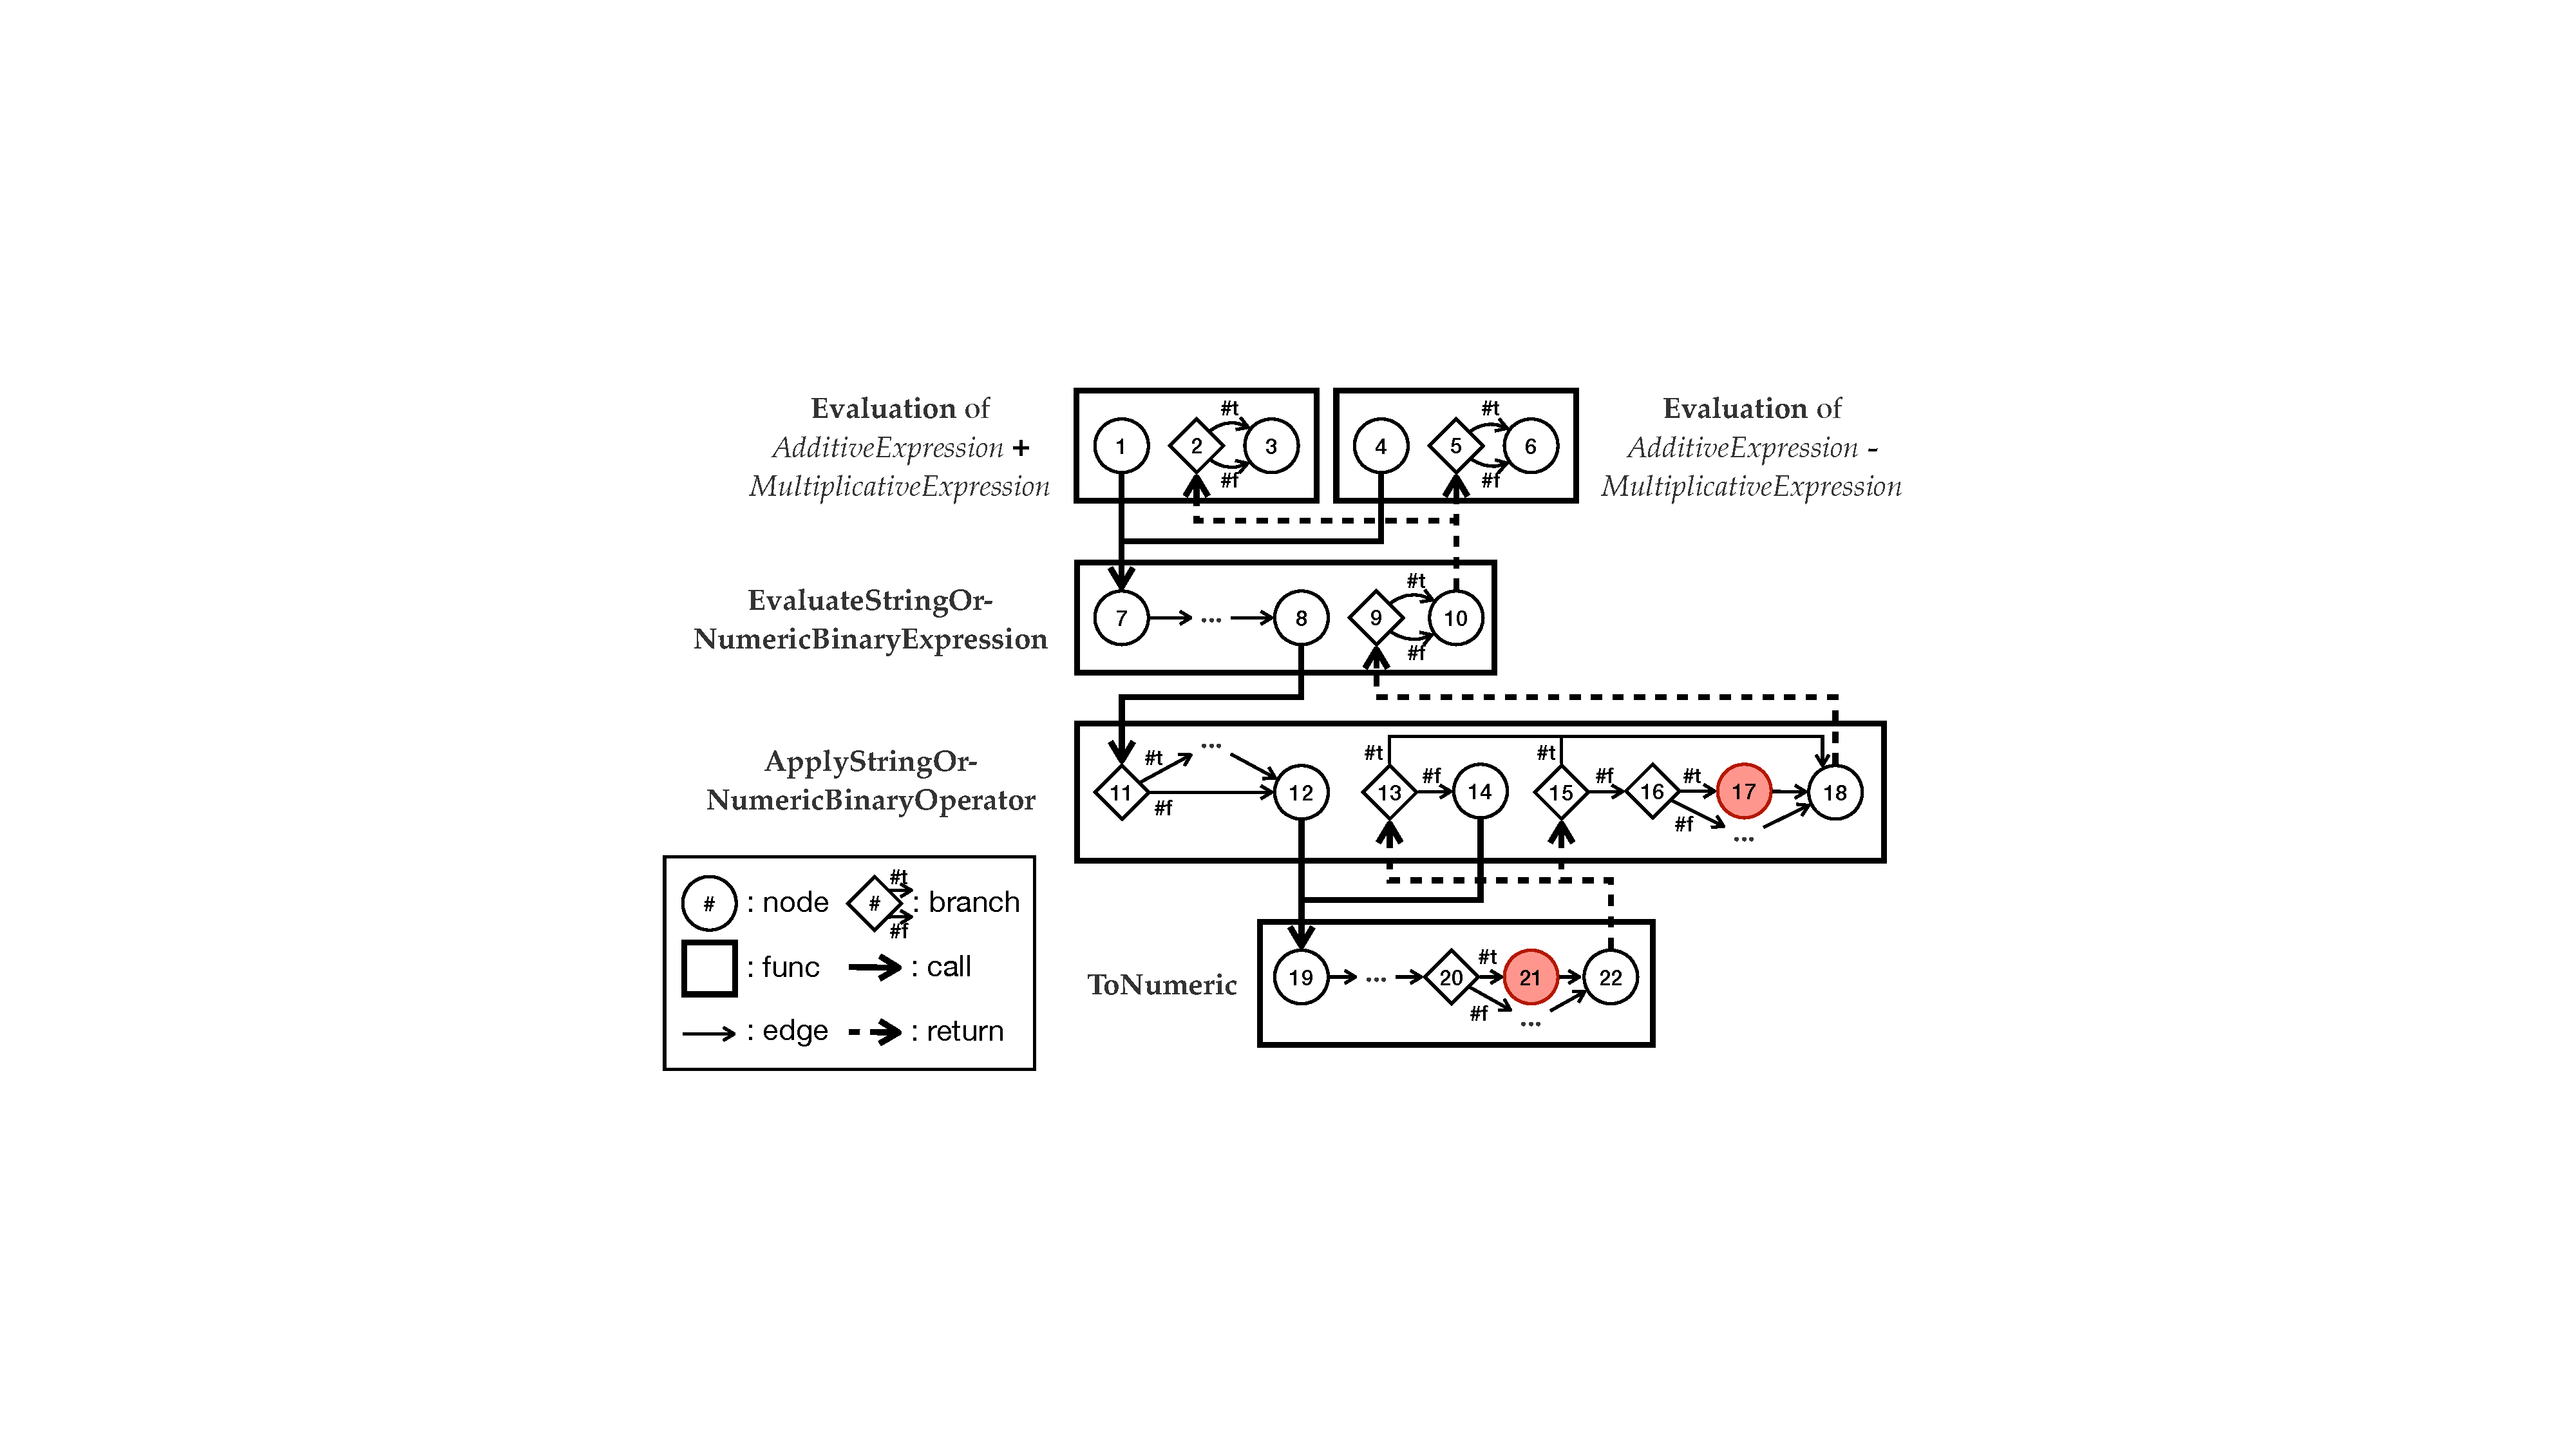
\includegraphics[width=0.87\textwidth]{img/spec-cfg}
  \caption{
    Control-flow graph (CFG) of abstract algorithms in
    Figures~\ref{fig:add-sdo}, \ref{fig:normal-algos}, and
    \ref{fig:builtin-number}
  }
  \label{fig:spec-cfg}
\vspace*{-1em}
\end{figure}

To define the coverage of a conformance test suite using graph coverage criteria,
we need a directed graph of the JavaScript mechanized specification.
CFG is the most common way to construct a directed
graph from a mechanized language specification.
In a CFG, a node denotes a sequence of instructions, and an edge
indicates a control flow in the mechanized specification.
An edge often has an annotation to represent a specific control flow,
such as conditional branches (\sname{\#t} or \sname{\#f}) and function calls
(\sname{call}) and returns (\sname{ret}).

For example, Figure~\ref{fig:spec-cfg} depicts a CFG of the abstract algorithms
in Figures~\ref{fig:add-sdo}, \ref{fig:normal-algos}, and
\ref{fig:builtin-number}.
In this figure, circles (or diamonds) denote nodes (or branches), arrows denote
edges, and boxes indicate algorithms.
The labels inside nodes match the labels annotated in the algorithms in
Figures~\ref{fig:add-sdo},~\ref{fig:normal-algos}, and~\ref{fig:builtin-number}.
Let us apply coverage-guided fuzzing~\cite{afl} with a node coverage
criterion in the CFG and assume that a simple JavaScript program, \jscode{1 + 2},
exists in the program pool.
It does not satisfy the condition in the branch labeled 20 because the left-hand and
right-hand sides of \jscode{1 + 2} are both Number values rather than BigInt values.
Thus, it does not cover the red node labeled 21.
Now assume that another program, \jscode{3n + 4n}, is generated by mutating
the previous program.
Then, it covers the red node labeled 21 because it satisfies the condition
in the branch labeled 20 with BigInt values on both sides of the \jscode{+} operator.

%----------------------------------------%
%----------------------------------------%

\subsection{Motivation}\label{sec:motiv}

Unfortunately, a simple node coverage criterion in CFGs of mechanized
specifications cannot fully discriminate different semantics in different
language features or even in the same feature.
We explain such cases with simple examples using the CFG in Figure~\ref{fig:spec-cfg}.

%----------------------------------------%
%----------------------------------------%

\subsubsection{Different Semantics in Different Language
Features}\label{sec:diff-feat}

The semantics of different language features may use the same abstract
algorithms as helper functions.
For example, the semantics of \scode{+} and \scode{-}
operators transitively use \textbf{ApplyStringOrNumericBinaryOperator}.
In the algorithm, the red node labeled 17 represents throwing
\textbf{TypeError} exception.
If the program pool contains a program \jscode{2n + 1}, it covers the red node
labeled 17 because it has different types of numeric values, a BigInt
\jscode{2n} and a Number \jscode{1}, as the left-hand and right-hand sides of the
\scode{+} operator.
Similarly, another program \jscode{2n - 1} using the \scode{-} operator
covers the node.
However, \jscode{2n - 1} will not be added to the program pool because
the node labeled 17 is already covered by \jscode{2n + 1},
even though \jscode{2n - 1} may reveal a different implementation of the semantics.
For a higher quality of conformance testing,
a more fine-grained definition of graph coverage is necessary
to discriminate \jscode{2n + 1} and \jscode{2n - 1}.

%----------------------------------------%
%----------------------------------------%

\subsubsection{Different Semantics in the Same Language
Feature}\label{sec:same-feat}
In addition, different parts in the semantics of the same language feature
may use the same algorithm more than once.
For example, the semantics of the \scode{+} operator uses
\textbf{ApplyStringOrNumericBinaryOperator}, and it invokes
\textbf{ToNumeric} twice in the nodes labeled 12 and 14.
Now, assume that the current program pool contains a program \jscode{2n + 1} again.
Then, the red node labeled 21 is covered by the program \jscode{2n + 1} because
the left-hand side is a BigInt \jscode{2n}.
It means that another similar program \jscode{1 + 2n} would not be added to the
program pool because the test requirement for a node labeled 21 is already covered
by \jscode{2n + 1}.
However, \jscode{1 + 2n} is also a meaningful test case because it checks the
edge case when the right-hand side of the \scode{+} operator is a BigInt value.

In the remainder of the paper, we formally define a feature-sensitive coverage
criterion and its variants to resolve the problems (Section~\ref{sec:fscov}).
Then, we explain how to implement a conformance test synthesizer with
feature-sensitive coverage criteria in Section~\ref{sec:impl}.
Finally, after evaluating feature-sensitive coverage criteria with
mainstream JavaScript implementations (Section~\ref{sec:eval}),
we discuss related work (Section~\ref{sec:related})
and conclude (Section~\ref{sec:conclusion}).

\section{Overview}\label{sec:overview}

\todo

\section{Feature-Sensitive Coverages}\label{sec:fscov}

This section first formulates the general definition of graph coverages for a
given directed graph and explains representative coverage metrics as examples.
%
Then, we introduce a \textit{feature-sensitive (FS) coverage} as a general
extension of graph coverages to fully discriminate semantics between different
language features.
%
Finally, we define a \textit{feature call path-sensitive (FCPS) coverage} as a
variant of FS coverage to distinguish different parts in the semantics of the
same language features.


%----------------------------------------%
%----------------------------------------%


\subsection{Notations}\label{sec:notation}
%
First, we define notations used in the definition of graph coverages.
%
A \textit{directed graph} $\graph = (\nodeset, \inodeset,
\fnodeset, \edgeset)$ consists of:
\begin{itemize}
  \item a set of \textit{nodes} $\nodeset$
  \item a set of \textit{initial nodes} $\inodeset \subseteq \nodeset$
  \item a set of \textit{final nodes} $\fnodeset \subseteq \nodeset$
  \item a set of \textit{edges} $\edgeset \subseteq \nodeset \times \nodeset
    \times (\annotset \uplus \{ \bot \})$ with a set of \textit{annotations}
    $\annotset$
\end{itemize}
%
The notation $\node \edge{\annot} \node'$ denotes an edge from a node $\node$ to
a node $\node'$ with an annotation $\annot \in \annotset$.
%
If an edge has an empty annotation $\bot$, we omit the annotation: $\node
\edge{} \node'$.
%
In a given directed graph $\graph$, a \textit{path} $\pat \in \patset{\graph}$
is a sequence of one or more nodes, where each pair of adjacent nodes is an
edge:
\begin{equation}\label{euq:path-def}
  \patset{\graph} = \{
    \node_0 \edge{\annot_0} \cdots \edge{\annot_{m-1}} \node_m \mid
    \forall i < m. \; \node_i \edge{\annot_i} \node_{i+1} \in \edgeset \wedge
    \node_m \in \nodeset
  \}
\end{equation}
%
The length of a path is defined as $\norm{\node_0 \edge{\annot_0} \cdots
\edge{\annot_{m-1}} \node_m} = m$.
%
A path $\pat$ is a \textit{subpath} ($\subpath$) of a path $\pat'$ when $\pat$
is a subsequence of $\pat'$.
%
We use the notation $\prefix$ for a prefix relation, and $\getfirst(\pat)$ and
$\getlast(\pat)$ denote the first and last nodes of the path $\pat$,
respectively.
%
A path $\pat$ is \textit{full} when it starts at an initial node and ends at a
final node: $\getfirst(\pat) \in \inodeset \wedge \getlast(\pat) \in \fnodeset$.
%
Then, $\patmap{\graph} : \testset \rightarrow \patset{\graph}$ is a mapping from
a \textit{test} $\test \in \testset$ to a full path in the graph $\graph$, and
we call $\patmap{\graph}(\test)$ as the \textit{execution path} of $\test$.

%----------------------------------------%

\paragraph{\textbf{Example}}
%
Consider a control-flow graph (CFG) $\graph$ depicted in
Figure~\ref{fig:spec-cfg} and the following JavaScript programs as a test set $T
\subseteq \testset$:
\begin{equation}\label{equ:testset}
  T = \left\{
    \begin{array}{rcl}
      \cdots\\
      \addtest &=& \text{(a JavaScript program \jscode{2n + 1;})}\\
      \subtest &=& \text{(a JavaScript program \jscode{2n - 1;})}\\
      \cdots\\
    \end{array}
  \right.
\end{equation}
%
Then, $\patmap{\graph}(\addtest)$ is the execution path of $\addtest$:
\[
  \small
  \!\begin{array}{l}
    \cdots
    \call \overset{\text{{\bf Evaluation} of \esnt{AdditiveExpression}
      \esconst{+} \esnt{MultiplicativeExpression}}}{\rcolorbox{gray3}{\(
    1
    \call
    \overset{\textbf{EvaluateStringOrNumericBinaryExpression}}{\rcolorbox{gray2}{\(
    7 \edge{} \cdots \edge{} 8
    \call \overset{\textbf{ApplyStringOrNumericBinaryOperator}}{\colorbox{gray1}{\(
    11 \edge{} \cdots \edge{} 12
    \call \overset{\textbf{ToNumeric}}{\colorbox{white}{\(
    19 \edge{} \cdots \edge{} 20 \tedge \colorbox{lightred}{21} \edge{} 22
    \)}}
    \ret 13 \fedge 14
    \)}}
    \)}}
    \)}}

    \vspace*{1em}\\

    \lcolorbox{gray3}{\(
    \lcolorbox{gray2}{\(
    \colorbox{gray1}{\(
    \call \overset{\textbf{ToNumeric}}{\colorbox{white}{\(
    19 \edge{} \cdots \edge{} 20 \fedge \cdots \edge{} 22
    \)}}
    \ret 15 \fedge 16 \tedge \colorbox{lightred}{17} \edge{} 18
    \)}
    \ret 9 \tedge 10
    \)}
    \ret 2 \tedge 3
    \)}
    \ret \cdots\\
  \end{array}
\]
And, $\patmap{\graph}(\subtest)$ is equal to $\patmap{\graph}(\addtest)$ except
for nodes 4, 5, and 6 in the $\textbf{Evaluation}$ SDO for subtraction rather
than 1, 2 and 3 in the $\textbf{Evaluation}$ SDO for addition.
%
The following path $\pat$ is a subpath of both $\patmap{\graph}(\addtest)$ and
$\patmap{\graph}(\subtest)$:
\begin{equation}\label{equ:subpath}
  \pat = 22 \ret 15 \fedge 16 \tedge \colorbox{lightred}{17}
\end{equation}
whose length is $\norm{\pat} = 3$.


%----------------------------------------%
%----------------------------------------%


\subsection{Graph Coverages}\label{sec:cov}

We formulate graph coverages by referring to their well-known
definitions~\cite{testing}.
%
For a given directed graph, we specify \textit{graph coverage} criteria by 1) a
set of \textit{test requirements} and 2) a \textit{cover relation} between paths
and test requirements:

%----------------------------------------%

\begin{definition}[Graph Coverage]\label{def:graph-cov}
  A \textit{graph coverage} criterion $\cov{\graph} = (\trset{\graph}, \cover)$
  for a given directed graph $\graph$ is defined with:
  \begin{itemize}
    \item a set of \textit{test requirements (TRs)} $\trset{\graph}$
    \item a \textit{cover relation} $\cover \subseteq \patset{\graph} \times
      \trset{\graph}$ between paths and TRs
  \end{itemize}
\end{definition}

%----------------------------------------%

In a specific graph coverage criterion $\cov{\graph}$, we say that a path $\pat$
\textit{covers} a TR $\tr \in \trset{\graph}$ when $\pat \cover
\tr$.
%
We also say that a test $\test \in \testset$ covers the TR $\tr$ if there exists
a prefix path $\pat$ of its execution path covers the TR:
%
\begin{equation}\label{equ:test-cover}
  \test \cover \tr
  \iff
  \exists \pat \in \patset{\graph}. \tst
  \pat \prefix \patmap{\graph}(\test) \wedge
  \pat \cover \tr
\end{equation}
%
A test set $T \subseteq \testset$ \textit{satisfies} ($\sat$) the criterion
$\cov{\graph}$ when it covers all valid TRs:
\begin{equation}\label{equ:sat}
  T \sat \cov{\graph}
  \iff
  \forall \tr \in \trset{\graph}. \;
  \tr \; \text{is valid} \; \Rightarrow
  \exists \test \in T. \tst \test \cover \tr
\end{equation}
where a TR $\tr$ is \textit{valid} if there exists a possible test $\test \in
\testset$ that covers $\tr$.
%
If $T \sat \cov{\graph} \Rightarrow T \sat \cov{\graph}'$ for any test set $T$,
we say that $\cov{\graph}$ \textit{subsumes} $\cov{\graph}'$ and use the
notation: $\cov{\graph} \subs \cov{\graph}'$.
%
The subsumption relation between graph coverage criteria is a partial order.

%----------------------------------------%

\begin{definition}[Node Coverage]\label{def:node-cov} In a \textit{node
  coverage} criterion $\nodecov{\graph}$,
  \begin{itemize}
    \item the set of \textbf{TRs} $\trset{\graph}$ is a set of nodes:
      \[
        \trset{\graph} = \nodeset
      \]
    \item a path $\pat$ \textbf{covers} a node $\node$ when it ends with the
      node $\node$:
      \[
        \pat \cover \node \iff \getlast(\pat) = \node
      \]
  \end{itemize}
\end{definition}

%----------------------------------------%

The node coverage is the most common graph coverage defined with nodes as test
requirements, and we could generalize it into \textit{$k$-limiting path
coverage} criteria using paths instead of nodes:

%----------------------------------------%

\begin{definition}[$k$-Limiting Path Coverage]\label{def:k-path-cov}
  In a \textit{$k$-limiting path coverage} criterion $\kpathcov{k}{\graph}$,
  \begin{itemize}
    \item the set of \textbf{TRs} $\trset{\graph}$ is a set of
      paths whose lengths are bounded by $k$:
      \[
        \trset{\graph} = \{ \pat \in \patset{\graph} \mid \norm{\pat} \leq k \}
      \]
    \item a path $\pat$ \textbf{covers} a path $\pat'$ when their last nodes are
      equal and the path $\pat'$ is a subpath of $\pat$:
      \[
        \pat \cover \pat'
        \iff
        \getlast(\pat) = \getlast(\pat') \wedge \pat' \subpath \pat
      \]
  \end{itemize}
\end{definition}

%----------------------------------------%

Now, a node coverage could be redefined as $0$-limiting path coverage
($\kpathcov{0}{\graph} = \nodecov{\graph}$), and other graph coverages are
defined with $k$-limiting path coverages as well:
\begin{itemize}
  \item An \textit{edge coverage} criterion is $\kpathcov{1}{\graph}$
  \item An \textit{edge-pair coverage} criterion is $\kpathcov{2}{\graph}$
  \item A \textit{complete path coverage} criterion is
    $\kpathcov{\infty}{\graph}$
\end{itemize}
%
Note that $k$-limiting path coverage criteria utilize the inequality for path
lengths $\norm{\pat} \leq k$ rather than equality $\norm{\pat} = k$.
%
Thus, if $i \leq j$, the set of TRs in $\kpathcov{i}{\graph}$ is always a subset
of that in $\kpathcov{j}{\graph}$, and $\kpathcov{j}{\graph}$ subsumes
$\kpathcov{i}{\graph}$.
%
A \textit{branch coverage} criterion is a variant of an edge coverage that
treats only out-edges of conditional branches as TRs.
%
It is possible to merge multiple coverage criteria by defining unions of TRs and
cover relations as the TR and cover relation of the merged coverage criterion.
%
For example, a \textit{node/branch coverage} criterion is a merged criterion of
node and branch coverage criteria.

%----------------------------------------%

A complete path coverage might have infinite TRs because of recursions and loop
structures.
%
To resolve this problem, \citet{testing} have presented a \textit{simple path
coverage} that deals with only simple paths as TRs.
%
A path $\node_0 \edge{\annot_0} \cdots \edge{\annot_{m-1}} \node_m$ is
\textit{simple} if no duplicated nodes in the path, with the exception that the
first and last nodes may be identical: $\forall i, j. \; \node_i = \node_j
\Rightarrow (i = j \vee \{ i, j \} = \{ 0, m \})$.
%
In addition, they extend it to a \textit{prime path coverage} to reduce the
number of TRs by filtering out meaningless simple paths.
%
It deals with only prime paths as TRs, where a \textit{prime path}
is a maximal length simple path in the graph.
%
However, such advanced structural coverage criteria still need a tremendous
number of TRs for the entire control-flow graphs.
%
Hence, they are commonly used only for unit testing~\cite{unit-test} in practice
with intra-procedural control-flow graphs.

%----------------------------------------%

\paragraph{\textbf{Example}}
%
Consider again a CFG $\graph$ depicted in Figure~\ref{fig:spec-cfg} and the test
set $T$ in (\ref{equ:testset}), including $\addtest$ and $\subtest$.
%
If we measure the $3$-limiting path coverage $\kpathcov{3}{\graph}$ for the test
set $T$, both a node 17 and the path $\pat$ in (\ref{equ:subpath}) are test
requirements $\trset{\graph}$.
%
First, the prefix path, whose last node is 17, of $\patmap{\graph}(\addtest)$
covers both TRs: node 17 and $\pat$.
%
Thus, the test $\addtest$ for addition covers both of them.
%
Similarly, the test $\subtest$ for subtraction covers both of them for the same
reason.
%
Unfortunately, it causes that either $\addtest$ or $\subtest$ might be removed
in the minimal test set because they cover the same TRs, node 17 and the path
$\pat$.


%----------------------------------------%
%----------------------------------------%


\subsection{Feature-Sensitive (FS) Coverages}\label{sec:fs-cov}

To alleviate the problem explained in Section~\ref{sec:diff-feat}, we introduce
a novel \textit{feature-sensitive (FS) coverage} as a general extension of any
graph coverages.
%
It depends on the following two components:
%
\begin{itemize}
  \item a set of \textit{language features} $\featset$
  \item a \textit{feature mapping} $\featmap: \nodeset \rightarrow \featset
    \uplus \{ \bot \}$, a partial mapping from nodes to language features.
\end{itemize}
%
where $\featmap(\node) = \bot$ means that there is no language feature for the
node $\node$.

%----------------------------------------%

We first define the \textit{call-site stack} $\css{\pat} \in \nodeset^*$ of a
path $\pat$ as a sequence of nodes constructed by:
\begin{equation}\label{equ:css}
  \css{\pat} = \left\{
    \begin{array}{ll}
      \epsilon &
      \tif \pat = \node\\

      {[\node_1, \cdots, \node_m, \getlast(\pat')]} &
      \tif \pat = \pat' \call \node \wedge
      \css{\pat'} = [\node_1, \cdots, \node_m]\\

      {[\node_1, \cdots, \node_{m-1}]} &
      \tif \pat = \pat' \ret \node \wedge
      \css{\pat'} = [\node_1, \cdots, \node_m]\\

      \css{\pat'} &
      \tif \pat = \pat' \edge{\annot} \node

    \end{array}
  \right.
\end{equation}
In other words, $\css{\pat}$ keeps only call-sites not matched with return-sites
in the path $\pat$.  A \textit{call-site} is a node having a call edge ($\call$)
as its out-edge, and a \textit{return-site} is a node having a return edge
($\ret$) as its in-edge.
%
Then, we define the \textit{feature extractor} $\extfeat: \css{\patset{\graph}}
\rightarrow \featset \uplus \{ \bot \}$ as a partial mapping from call-site
stacks to enclosing language features $\featset$:
\begin{equation}\label{equ:extfeat}
  \extfeat([\node_1, \cdots, \node_m]) = \left\{
    \begin{array}{ll}
      \feat & \tif
      \exists i. \tst \featmap(\node_i) = \feat \wedge
      \forall j > i. \; \featmap(\node_j) = \bot
      \\

      \bot & \telse
    \end{array}
  \right.
\end{equation}
%
Similarly, $\extfeat(\css{\pat}) = \bot$ means that there is no language feature
for the path $\pat$.

%----------------------------------------%

\begin{definition}[Feature-Sensitive (FS) Coverage]\label{def:fs-cov}
  For a given graph coverage $\cov{\graph} = (\trset{\graph}, \cover)$, the
  \textit{feature-sensitive (FS) coverage} $\fcov{\graph} = (\ftrset{\graph},
  \cover)$ is defined as follows:
  \begin{itemize}
    \item the set of \textbf{feature-sensitive test requirements (FS-TRs)}
      $\ftrset{\graph}$ is a set of original TRs optionally tagged with language
      features:
      \[
        \ftrset{\graph} = \trset{\graph} \times (\featset \uplus \{ \bot \})
      \]
    \item a path $\pat$ \textbf{covers} a FS-TR $(\tr, \feat)$ when $\pat$
      covers the original TR $\tr$ and $\feat$ is the enclosing language feature
      of $\pat$:
      \[
        \pat \cover (\tr, \feat) \iff \pat \cover \tr \wedge
        \extfeat(\css{\pat}) = \feat
      \]
  \end{itemize}
\end{definition}

%----------------------------------------%

\paragraph{\textbf{Example}}
%
For the CFG $\graph$ depicted in Figure~\ref{fig:spec-cfg}, we could define the
feature mapping $\featmap$ as follows:
\begin{equation}\label{equ:featmap}
  \featmap(\node) = \left\{
    \begin{array}{ll}
      \addfeat & \tif \node \in \{ 1, 2, 3\} \\
      \subfeat & \tif \node \in \{ 4, 5, 6\} \\
      \numfeat & \tif \node \in \{ 23, 24, 25, 26 \} \\
      \bot & \telse
    \end{array}
  \right.
\end{equation}
%
Consider two tests $\addtest$ and $\subtest$ in the test set $T$
(\ref{equ:testset}), and two prefix paths $\addpat$ and $\subpat$, whose last
nodes are 17, of their execution paths:
%
\begin{equation}\label{equ:prepath}
  \begin{array}{rclcl}
    \addpat &=& \cdots \tedge 17 &\tst&
    \addpat \prefix \patmap{\graph}(\addtest)\\

    \subpat &=& \cdots \tedge 17 &\tst&
    \subpat \prefix \patmap{\graph}(\subtest)\\
  \end{array}
\end{equation}
%
First, the call-site stack of $\addpat$ is $\css{\addpat} = [\cdots, 1, 8]$
because other call-sites 12 and 14 are removed by matched return-sites 13 and
15, respectively.
%
Since there is no feature mapping for the call-site 8, the enclosing language
feature of $\addpat$ is $\extfeat(\css{\addpat}) = \featmap(1) = \addfeat$.
%
Hence, if we use a FS node coverage $\fnodecov{\graph}$, the path $\addpat$
covers a FS-TS $(17, \addfeat)$, and the test $\addtest$ for addition covers it
as well.
%
In a similar way, we know that the enclosing language feature of $\subpat$
is $\extfeat(\css{\subpat}) = \featmap(4) = \subfeat$.
%
It means that $\subtest$ covers a new FS-TS $(17, \subfeat)$ instead of $(17,
\addfeat)$ and remains in the minimal test set.

%----------------------------------------%

In addition, we extend the feature extractor $\extfeat$ to apply $k$-limiting
approach to FS coverages. The extended feature extractor $\extfeats{k}:
\css{\patset{\graph}} \rightarrow \featset^{\leq k}$ collects at most $k$
enclosing language features:
%
\begin{equation}\label{equ:extfeats}
  \extfeats{k}([\node_1, \cdots, \node_m]) = \left\{
    \begin{array}{ll}
      \epsilon & \tif k = 0 \vee m = 0\\

      \extfeats{k-1}([\node_1, \cdots, \node_{m-1}]) + \feat & \tif
      \featmap(\node_m) = \feat\\

      \extfeats{k}([\node_1, \cdots, \node_{m-1}]) & \telse\\
    \end{array}
  \right.
\end{equation}

%----------------------------------------%

\begin{definition}[$k$-Limiting Feature-Sensitive ($k$-FS)
  Coverage]\label{def:k-fs-cov}
  For a given graph coverage $\cov{\graph} = (\trset{\graph}, \cover)$, the
  \textit{$k$-limiting feature-sensitive ($k$-FS) coverage} $\kfcov{k}{\graph} =
  (\kftrset{k}{\graph}, \cover)$ is defined as follows:
  \begin{itemize}
    \item the set of \textbf{$k$-feature-sensitive test requirements
      ($k$-FS-TRs)} $\kftrset{k}{\graph}$ is a set of original TRs tagged with
      at most $k$ language features:
      \[
        \kftrset{k}{\graph} = \trset{\graph} \times \featset^{\leq k}
      \]
    \item a path $\pat$ \textbf{covers} a $k$-FS-TR $(\tr, \feats)$ when $\pat$
      covers the original TR $\tr$ and $\feats$ is the $k$-most enclosing
      language features of $\pat$:
      \[
        \pat \cover (\tr, \feats) \iff \pat \cover \tr \wedge
        \extfeats{k}(\css{\pat}) = \feats
      \]
  \end{itemize}
\end{definition}

%----------------------------------------%

\paragraph{\textbf{Example}}
%
Now, consider the following JavaScript program as a test $\test$ with the graph
in Figure~\ref{fig:spec-cfg}:
\[
  \begin{array}{rcl}
    \test \in \testset &=&
    \text{(a JavaScript program \jscode{[] - (2n + 1);})}\\
  \end{array}
\]
Then, it throws a \textbf{TypeError} exception in node 17 during the execution
of the expression \jscode{2n + 1}.
%
Consider the prefix path $\pat$, whose last node is 17, of the execution path of
$\test$.
%
Then, $\extfeats{2}(\pat) = [\subfeat, \addfeat]$ because the most enclosing
language feature is $\addfeat$, and the next enclosing one is $\subfeat$ for the
path $\pat$.
%
If we use $2$-FC node coverage $\kfnodecov{2}{\graph}$, the set of $2$-FS-TRs is
$\kftrset{2}{\graph} = (\nodeset, \featset^{\leq 2})$, and the test $\test$
covers a $2$-FS-TR $(17, [\subfeat, \addfeat])$.

%----------------------------------------%

The $k$-FS coverage divides TRs using each combination of different language
features.
%
Especially, the $k$-FS coverage with $k > 2$ is helpful to cover edge cases in
JavaScript engines and transpilers because they are heavily optimized and handle
even same language features differently depending on which language features are
used together.
%
For example, a \jscode{let} declaration just declares a block-scoped local
variable.
%
However, JavaScript engines and transpilers often have a different execution path
to handle it when it is declared in a \jscode{for-in/of} statement rather than a
simple block.
%
Indeed, the GraalJS~\cite{graaljs} engine and the Babel~\cite{babel} transpiler
contain conformance and crashing bugs only reproducible with a combination of
\jscode{let} declaration and \jscode{for-in/of} statement.\footnote{
  See \url{https://github.com/oracle/graaljs/issues/656} and
  \url{https://github.com/babel/babel/issues/15100}
}

%----------------------------------------%
%----------------------------------------%

\subsection{Feature Call Path-Sensitive (FCPS) Coverages}\label{sec:fcps-cov}

As explained in Section~\ref{sec:same-feat}, a more fine-grained set of test
requirements is necessary to distinguish different parts of the semantics even
in the same language features.
%
To resolve this problem, we define a \textit{feature call path-sensitive (FCPS)
coverage} as a variant of FS coverage.
%
The main idea of FCPS coverage is to distinguish TRs using paths from the most
enclosing language features.
%
However, if we keep paths as it is, the number of TRs exponentially increases
because of the path explosion caused by sequential branches.
%
Hence, we simplify a path $\pat$ to a corresponding \textit{feature call path}
$\fcp \in \fcpset = \featset \times \css{\patset{\graph}}$, which consists of
the most enclosing feature and a subsequence of the call-site stack
$\css{\pat}$ from the feature.
%
We define the \textit{feature call path extractor} $\extfcp:
\css{\patset{\graph}} \rightarrow (\fcpset \uplus \{ \bot \})$ as follows:
%
\begin{equation}\label{equ:extfcp}
  \extfcp([\node_1, \cdots, \node_m]) = \left\{
    \begin{array}{ll}
      \bot & \tif m = 0\\

      (\feat, [\node_m]) & \tif \featmap(\node_m) = \feat\\

      \fcp & \tif \fcp = \bot\\

      (\feat, [\node'_0, \cdots, \node'_i]) &
      \tif \fcp = (\feat, [\node'_0, \cdots, \node'_{m'}]) \wedge
      \exists i. \tst \node'_i = \node_m\\

      (\feat, \nodes + \node_m) & \tif \fcp = (\feat, \nodes)\\
    \end{array}
  \right.
\end{equation}
%
where $\fcp = \extfcp([\node_1, \cdots, \node_{m-1}])$.
%
Initially, this algorithm starts with $\bot$, which denotes no feature call path
for $\pat$, because there is no enclosing feature in the beginning ($m = 0$).
%
Then, it recursively keeps the call-sites in a given call-site
stack $\css{\pat}$.
%
However, it refreshes the result when there exists a mapping from the current
call-site to a language feature ($\featmap(\node_m) = \feat$).
%
In addition, it removes cycles in the result to prevent a possibly infinite
length of feature call path and remove the meaningless cases ($\exists i. \tst
\node'_i = \node_m$).

%----------------------------------------%

\begin{definition}[Feature Call Path-Sensitive (FCPS)
  Coverage]\label{def:fcps-cov}
  For a given graph coverage $\cov{\graph} = (\trset{\graph}, \cover)$, the
  \textit{feature call path-sensitive (FCPS) coverage} $\fcov{\graph} =
  (\fcptrset{\graph}, \cover)$ is defined as follows:
  \begin{itemize}
    \item the set of \textbf{feature call path-sensitive test requirements
      (FCPS-TRs)} $\fcptrset{\graph}$ is a set of original TRs optionally tagged
      with feature call paths.
      \[
        \fcptrset{\graph} = \trset{\graph} \times (\fcpset \uplus \{ \bot \})
      \]
    \item a path $\pat$ \textbf{covers} a FCPS-TR $(\tr, \fcp)$ when $\pat$
      covers the original TR $\tr$ and $\fcp$ is the feature call path extracted
      from $\pat$:
      \[
        \pat \cover (\tr, \fcp) \iff \pat \cover \tr \wedge
        \extfcp(\css{\pat}) = \fcp
      \]
  \end{itemize}
\end{definition}

%----------------------------------------%

\paragraph{\textbf{Example}}

\begin{figure}
  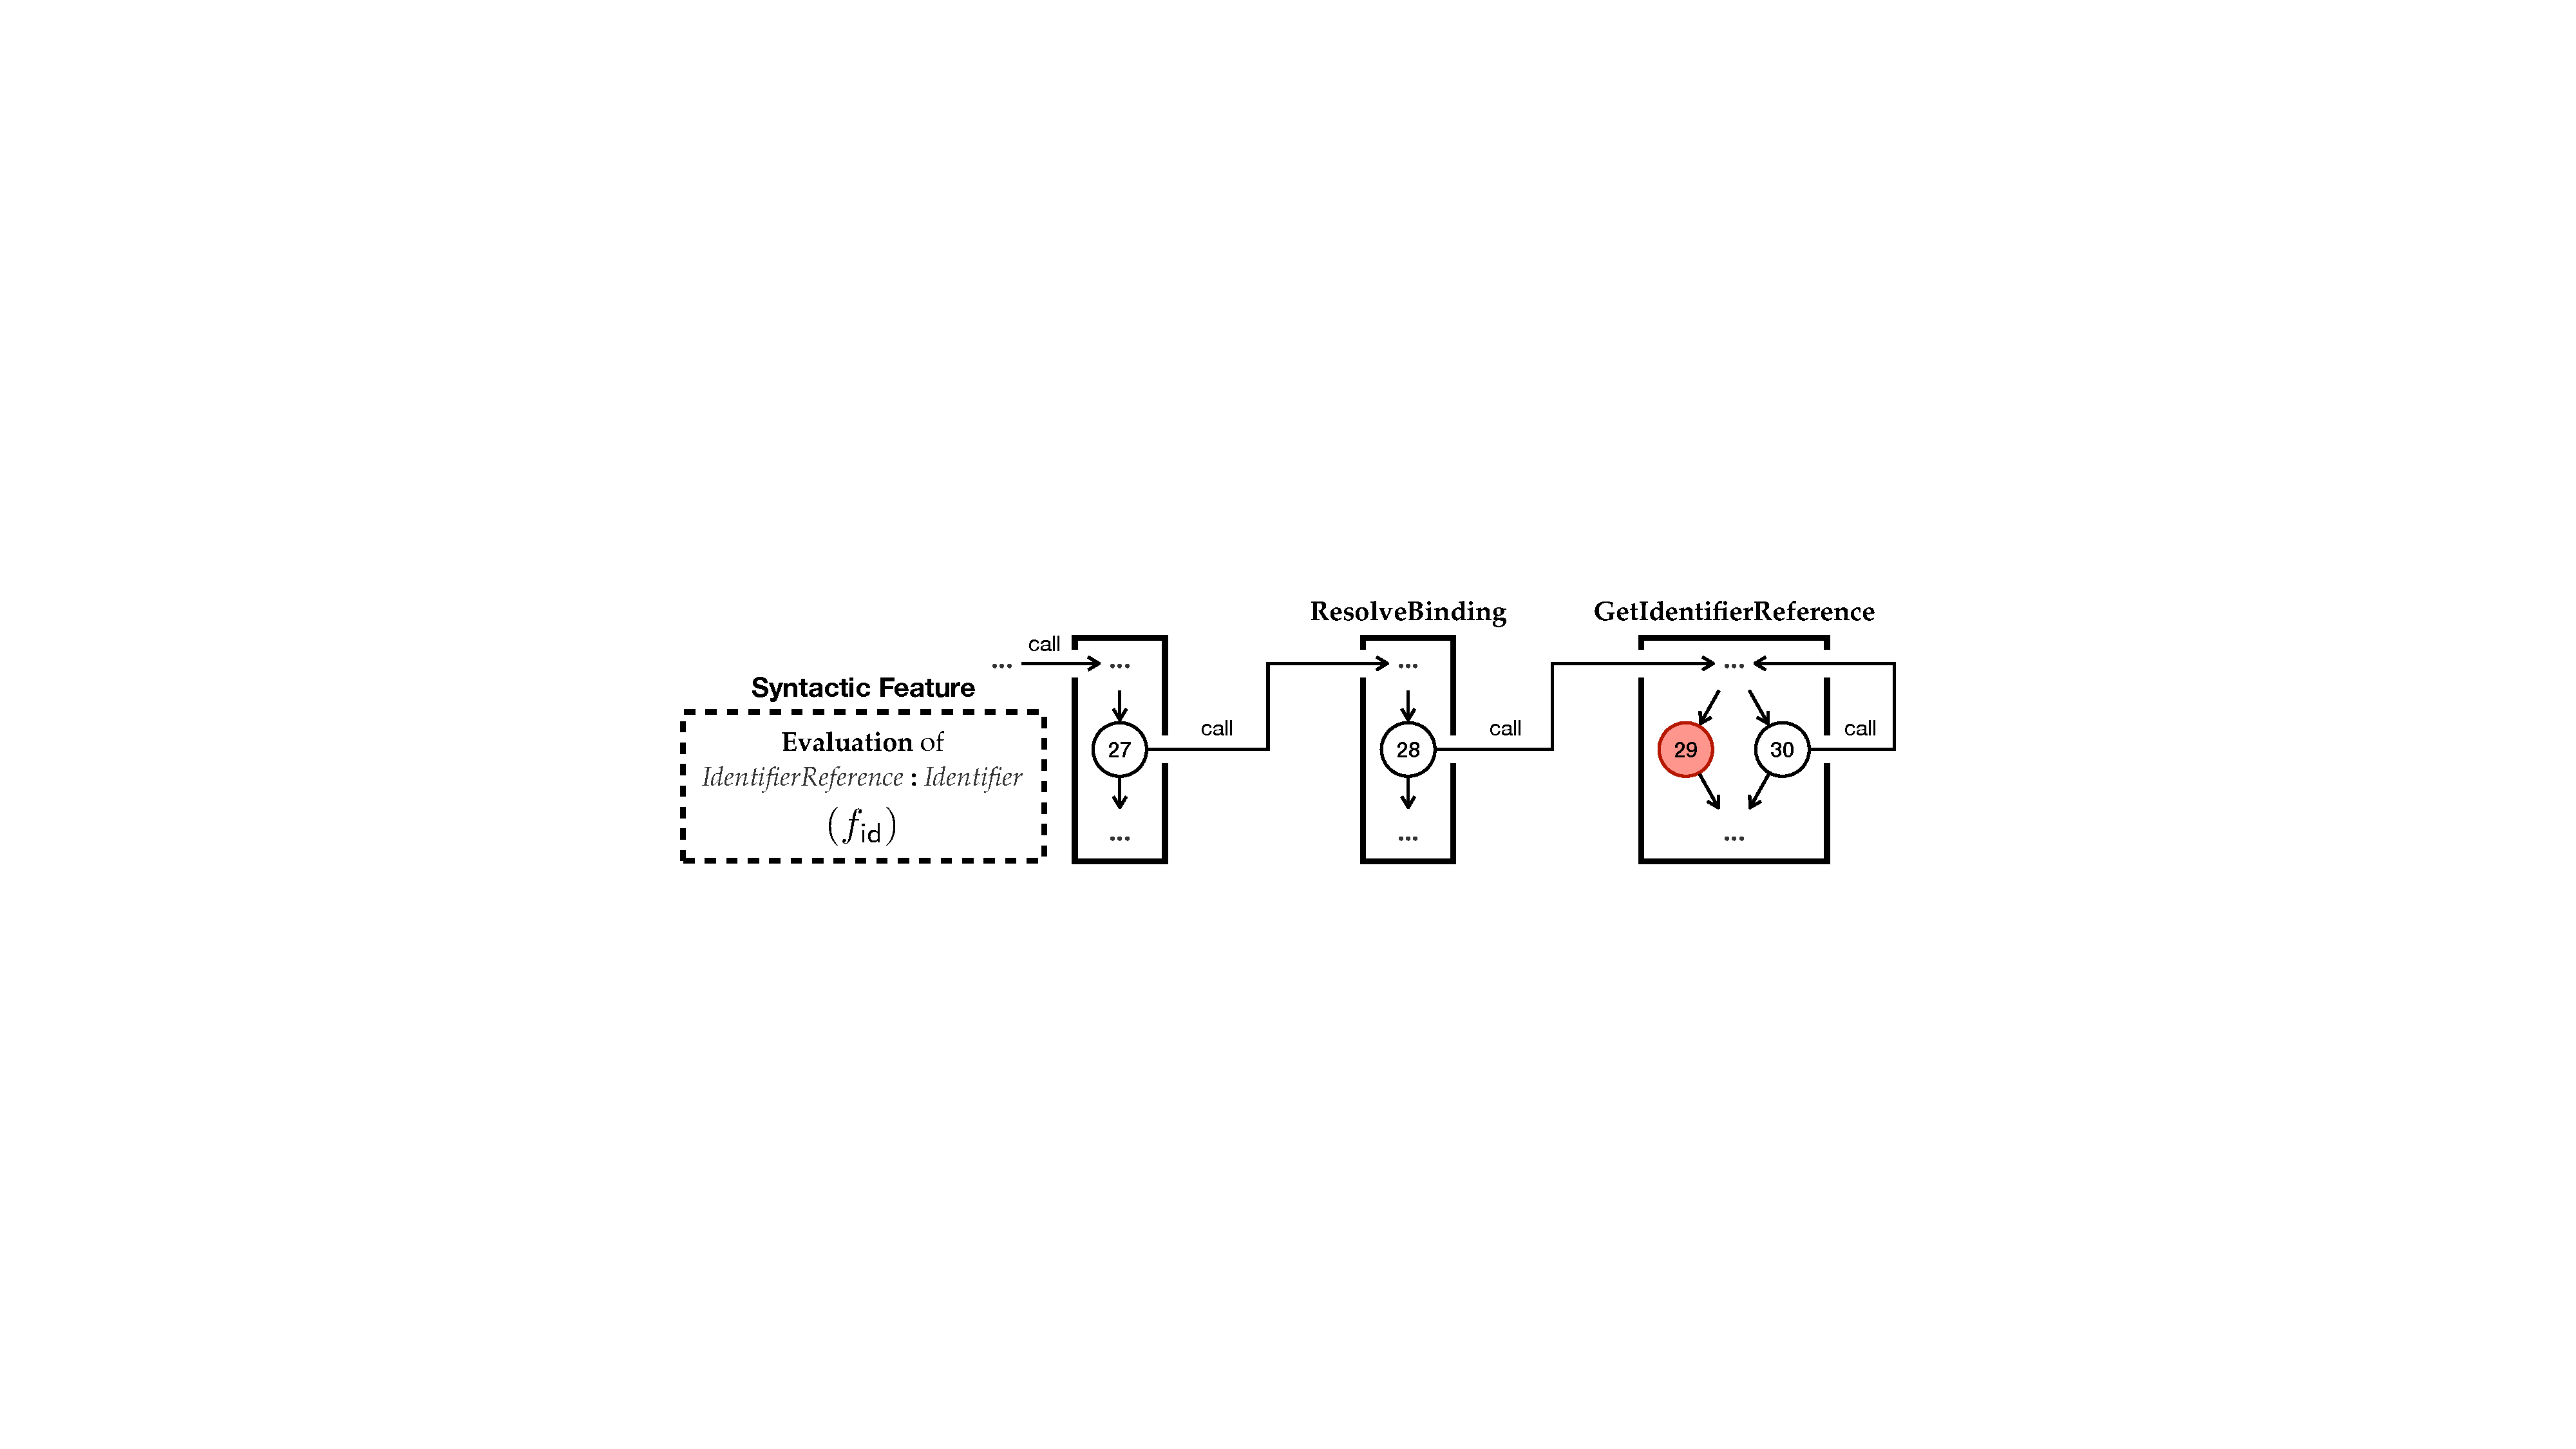
\includegraphics[width=0.85\textwidth]{img/spec-cfg-id}
  \caption{
    An excerpt from the CFG of abstract algorithms in ES13 related to $\idfeat$,
    a syntactic feature defined by the first alternative of
    \esnt{IdentifierReference} and its \textbf{Evaluation} SDO.
  }
  \label{fig:spec-cfg-id}
\end{figure}

We show two examples for FCPS node coverages in graph with graphs in
Figure~\ref{fig:spec-cfg} and Figure~\ref{fig:spec-cfg-id}.
%
First, consider the following two JavaScript programs as tests with the CFG in
Figure~\ref{fig:spec-cfg}:
%
\begin{equation}\label{equ:fcps-example1}
  \begin{array}{rcl}
    \test_0 \in \testset &=& \text{(a JavaScript program \jscode{2n + 1;})}\\
    \test_1 \in \testset &=& \text{(a JavaScript program \jscode{1 + 2n;})}\\
  \end{array}
\end{equation}
%
If we use FS node coverage, both tests $\test_0$ and $\test_1$ cover the same
FS-TR $(21, \addfeat)$, and one of them might be removed in the minimal test
set.
%
However, if we use FCPS node coverage, $\test_0$ and $\test_1$ cover different
FCPS-TRs $(21, (\addfeat, [1, 8, 12]))$ and $(21, (\addfeat, [1, 8, 14]))$,
respectively.
%
The other example is about the cycles in the call-site stacks with the graph in
Figure~\ref{fig:spec-cfg-id}.
%
It depicts an excerpt from the CFG of abstract algorithms in ES13 related to
$\idfeat$, a syntactic feature defined by the first alternative of
\esnt{IdentifierReference} and its \textbf{Evaluation} SDO. 
%
Assume that we do not remove cycles in the feature call paths $\fcpset$ during
the extraction algorithm $\extfcp$.
%
Then, since the algorithm \textbf{GetIdentifierReference} contains a
self-recursion, there exists an infinite number of possible feature call paths
from $\idfeat$ to node 29:
%
\begin{equation}\label{fcp-inf-example}
  (\idfeat, [27, 28]) \qquad
  (\idfeat, [27, 28, 30]) \qquad
  (\idfeat, [27, 28, 30, 30]) \qquad
  \cdots
\end{equation}
%
However, we remove cycles in feature call paths to resolve this issue, and there
exists only two possible feature call paths: $(\idfeat, [27, 28])$ and
$(\idfeat, [27, 28, 30])$.

%----------------------------------------%

Similar to the extension of FS coverages to $k$-FS coverages, we define a
$k$-FCPS coverage by extending the $\extfcp$ into $\extfcps{k}:
\css{\patset{\graph}} \rightarrow \fcpset^{\leq k}$ where $\fcpset^{\leq k} =
\featset^{\leq k} \times \css{\patset{\graph}}$:
%
\begin{equation}\label{equ:extfcps}
  \extfcps{k}([\node_1, \cdots, \node_m]) = \left\{
    \begin{array}{ll}
      (\epsilon, \epsilon) & \tif k = 0 \vee m = 0\\

      (\feats + \feat, [\node_m]) & \tif \featmap(\node_m) = \feat \wedge
      \extfcps{k-1}([\node_1, \cdots, \node_{m-1}]) = (\feats, \_)\\

      \fcps & \tif \fcps = (\epsilon, \epsilon)\\

      (\feats, [\node'_0, \cdots, \node'_i]) &
      \tif \fcp = (\feats, [\node'_0, \cdots, \node'_{m'}]) \wedge
      \exists i. \tst \node'_i = \node_m\\

      (\feats, \nodes + \node_m) & \tif \fcp = (\feats, \nodes)\\
    \end{array}
  \right.
\end{equation}
%
where $\fcps = \extfcps{k}([\node_1, \cdots, \node_{m-1}])$.

%----------------------------------------%

\begin{definition}[$k$-Limiting Feature Call Path-Sensitive ($k$-FCPS)
  Coverage]\label{def:k-fcps-cov}
  For a given graph coverage $\cov{\graph} = (\trset{\graph}, \cover)$, the
  \textit{$k$-limiting feature call path-sensitive ($k$-FCPS) coverage}
  $\kfcpcov{k}{\graph} = (\kfcptrset{k}{\graph}, \cover)$ is defined as follows:
  \begin{itemize}
    \item the set of \textbf{$k$-feature call path-sensitive test requirements
      ($k$-FCPS-TRs)} $\kfcptrset{k}{\graph}$ is a set of original TRs tagged
      with extends feature call paths bounded by $k$:
      \[
        \kfcptrset{k}{\graph} = \trset{\graph} \times \fcpset^{\leq k}
      \]
    \item a path $\pat$ \textbf{covers} a $k$-FCPS-TR $(\tr, \fcps)$ when $\pat$
      covers the original TR $\tr$ and $\fcps$ is the extended feature call path
      extracted from $\pat$:
      \[
        \pat \cover (\tr, \fcps) \iff \pat \cover \tr \wedge
        \extfcps{k}(\css{\pat}) = \fcps
      \]
  \end{itemize}
\end{definition}

%----------------------------------------%

\begin{figure}
  \centering
  \small
  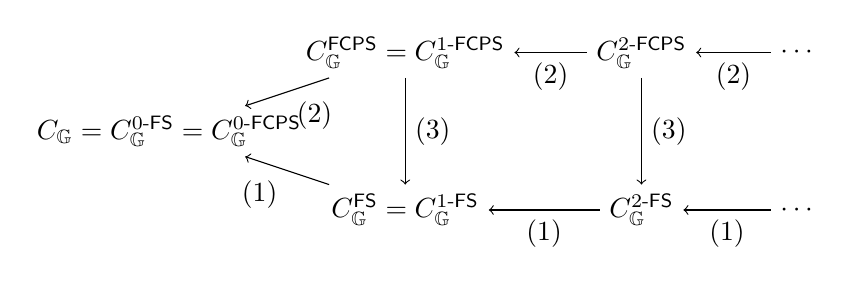
\begin{tikzpicture}[every node/.style={draw=none}]
    \node (base)   at (0,1) {$\cov{\graph}=\kfcov{0}{\graph}=\kfcpcov{0}{\graph}$};
    \node (1-fs)   at (3,0) {$\fcov{\graph}=\kfcov{1}{\graph}$};
    \node (2-fs)   at (6,0) {$\kfcov{2}{\graph}$};
    \node (k-fs)   at (8,0) {$\cdots$};
    \node (1-fcps) at (3,2) {$\fcpcov{\graph}=\kfcpcov{1}{\graph}$};
    \node (2-fcps) at (6,2) {$\kfcpcov{2}{\graph}$};
    \node (k-fcps) at (8,2) {$\cdots$};
    \path[->]
    (1-fs) edge node[auto] {(1)} (base)
    (2-fs) edge node[auto] {(1)} (1-fs)
    (k-fs) edge node[auto] {(1)} (2-fs)
    (1-fcps) edge node[auto] {(2)} (base)
    (1-fcps) edge node[auto] {(3)} (1-fs)
    (2-fcps) edge node[auto] {(2)} (1-fcps)
    (2-fcps) edge node[auto] {(3)} (2-fs)
    (k-fcps) edge node[auto] {(2)} (2-fcps);
  \end{tikzpicture}
  \caption{
    The subsumption relations between $k$-FS and $k$-FCPS coverages.
  }
  \label{fig:subs}
\end{figure}

In addition, we prove Theorem~\ref{thm:subs} for the subsumption relations
between $k$-FS and $k$-FCPS coverages.
%
We first prove the Lemma~\ref{lem:subs} and prove the theorem using it.
%
Figure~\ref{fig:subs} depicts the subsumption relations between them using edges
annotated with the corresponding equation in Theorem~\ref{thm:subs}.

%----------------------------------------%

\begin{lemma}\label{lem:subs}
  Consider two graph coverages $\cov{\graph} = (\trset{\graph}, \cover)$ and
  $\cov{\graph}' = (\trset{\graph}', \cover')$.
  %
  If there exists a valid TR $\tr \in \trset{\graph}$ that satisfies the following
  condition for each valid TR $\tr' \in \trset{\graph}'$:
  %
  \begin{equation}\label{equ:subs-lemma}
    \forall \test \in \testset. \; \test \cover \tr \Rightarrow \test \cover' \tr'
  \end{equation}
  %
  Then, $\cov{\graph}$ subsumes $\cov{\graph}'$ ($\cov{\graph}
  \subs\cov{\graph}'$).
\end{lemma}
\begin{proof}
  Assume $T \sat \cov{\graph}$.
  %
  For a given valid TR $\tr' \in \trset{\graph}'$, let $\tr \in \trset{\graph}$
  be the valid TR satisfies (\ref{equ:subs-lemma}).
  %
  Then, there exists a test $\test \in T$ such that $\test \cover \tr$ because
  $\tr$ is valid and $T \sat \cov{\graph}$.
  %
  Finally, $\test \cover \tr'$ because of (\ref{equ:subs-lemma}).
\end{proof}

\begin{theorem}[Subsumption Relation]\label{thm:subs}
  For a given integer $k > 0$, the following three subsumption relations
  ($\subs$) between $k$-FS and $k$-FCPS coverages satisfy:
  \begin{enumerate}
    \item $\kfcov{k}{\graph} \subs \kfcov{(k-1)}{\graph}$
    \item $\kfcpcov{k}{\graph} \subs \kfcpcov{(k-1)}{\graph}$
    \item $\kfcpcov{k}{\graph} \subs \kfcov{k}{\graph}$
  \end{enumerate}
\end{theorem}

\begin{proof}
  We prove the first subsumption relation using Lemma~\ref{lem:subs}, but omit
  the other second and third ones because it is possible to prove them in a
  similar way.
  %
  Let $k > 0$.
  %
  For a given valid $(k-1)$-FS-TR $(\tr, \feats)$, there exists a test $\test
  \in \testset$ such that $\test \cover (\tr, \feats)$ because $(\tr, \feats)$
  is valid.
  %
  There exists a prefix path $\pat$ of $\patmap{\graph}(\test)$ such that $\pat
  \cover (\tr, \feats)$ ($\because$ (\ref{equ:test-cover}))
  %
  Then, a $k$-FS-TR $(\tr, \extfeats{k}(\css{\pat}))$ satisfies the condition
  (\ref{equ:subs-lemma}) because of the inductive definition of $\extfeats{k}$
  in (\ref{equ:extfeats}).
  %
  Hence, $k$-FS coverages subsumes $(k-1)$-FS coverages.
\end{proof}

\section{Implementation}\label{sec:impl}

This section introduces our implementation $\tool$, an extension of a
state-of-the-art JavaScript conformance test synthesizer $\jest$~\cite{jest},
that supports both $k$-FS and $k$-FCPS coverage criteria.
%
Then, we explain how to detect conformance in JavaScript engines and transpilers
using the synthesized conformance tests.

%----------------------------------------%
%----------------------------------------%

\subsection{Overall Structure}\label{sec:overall}

\begin{figure}
  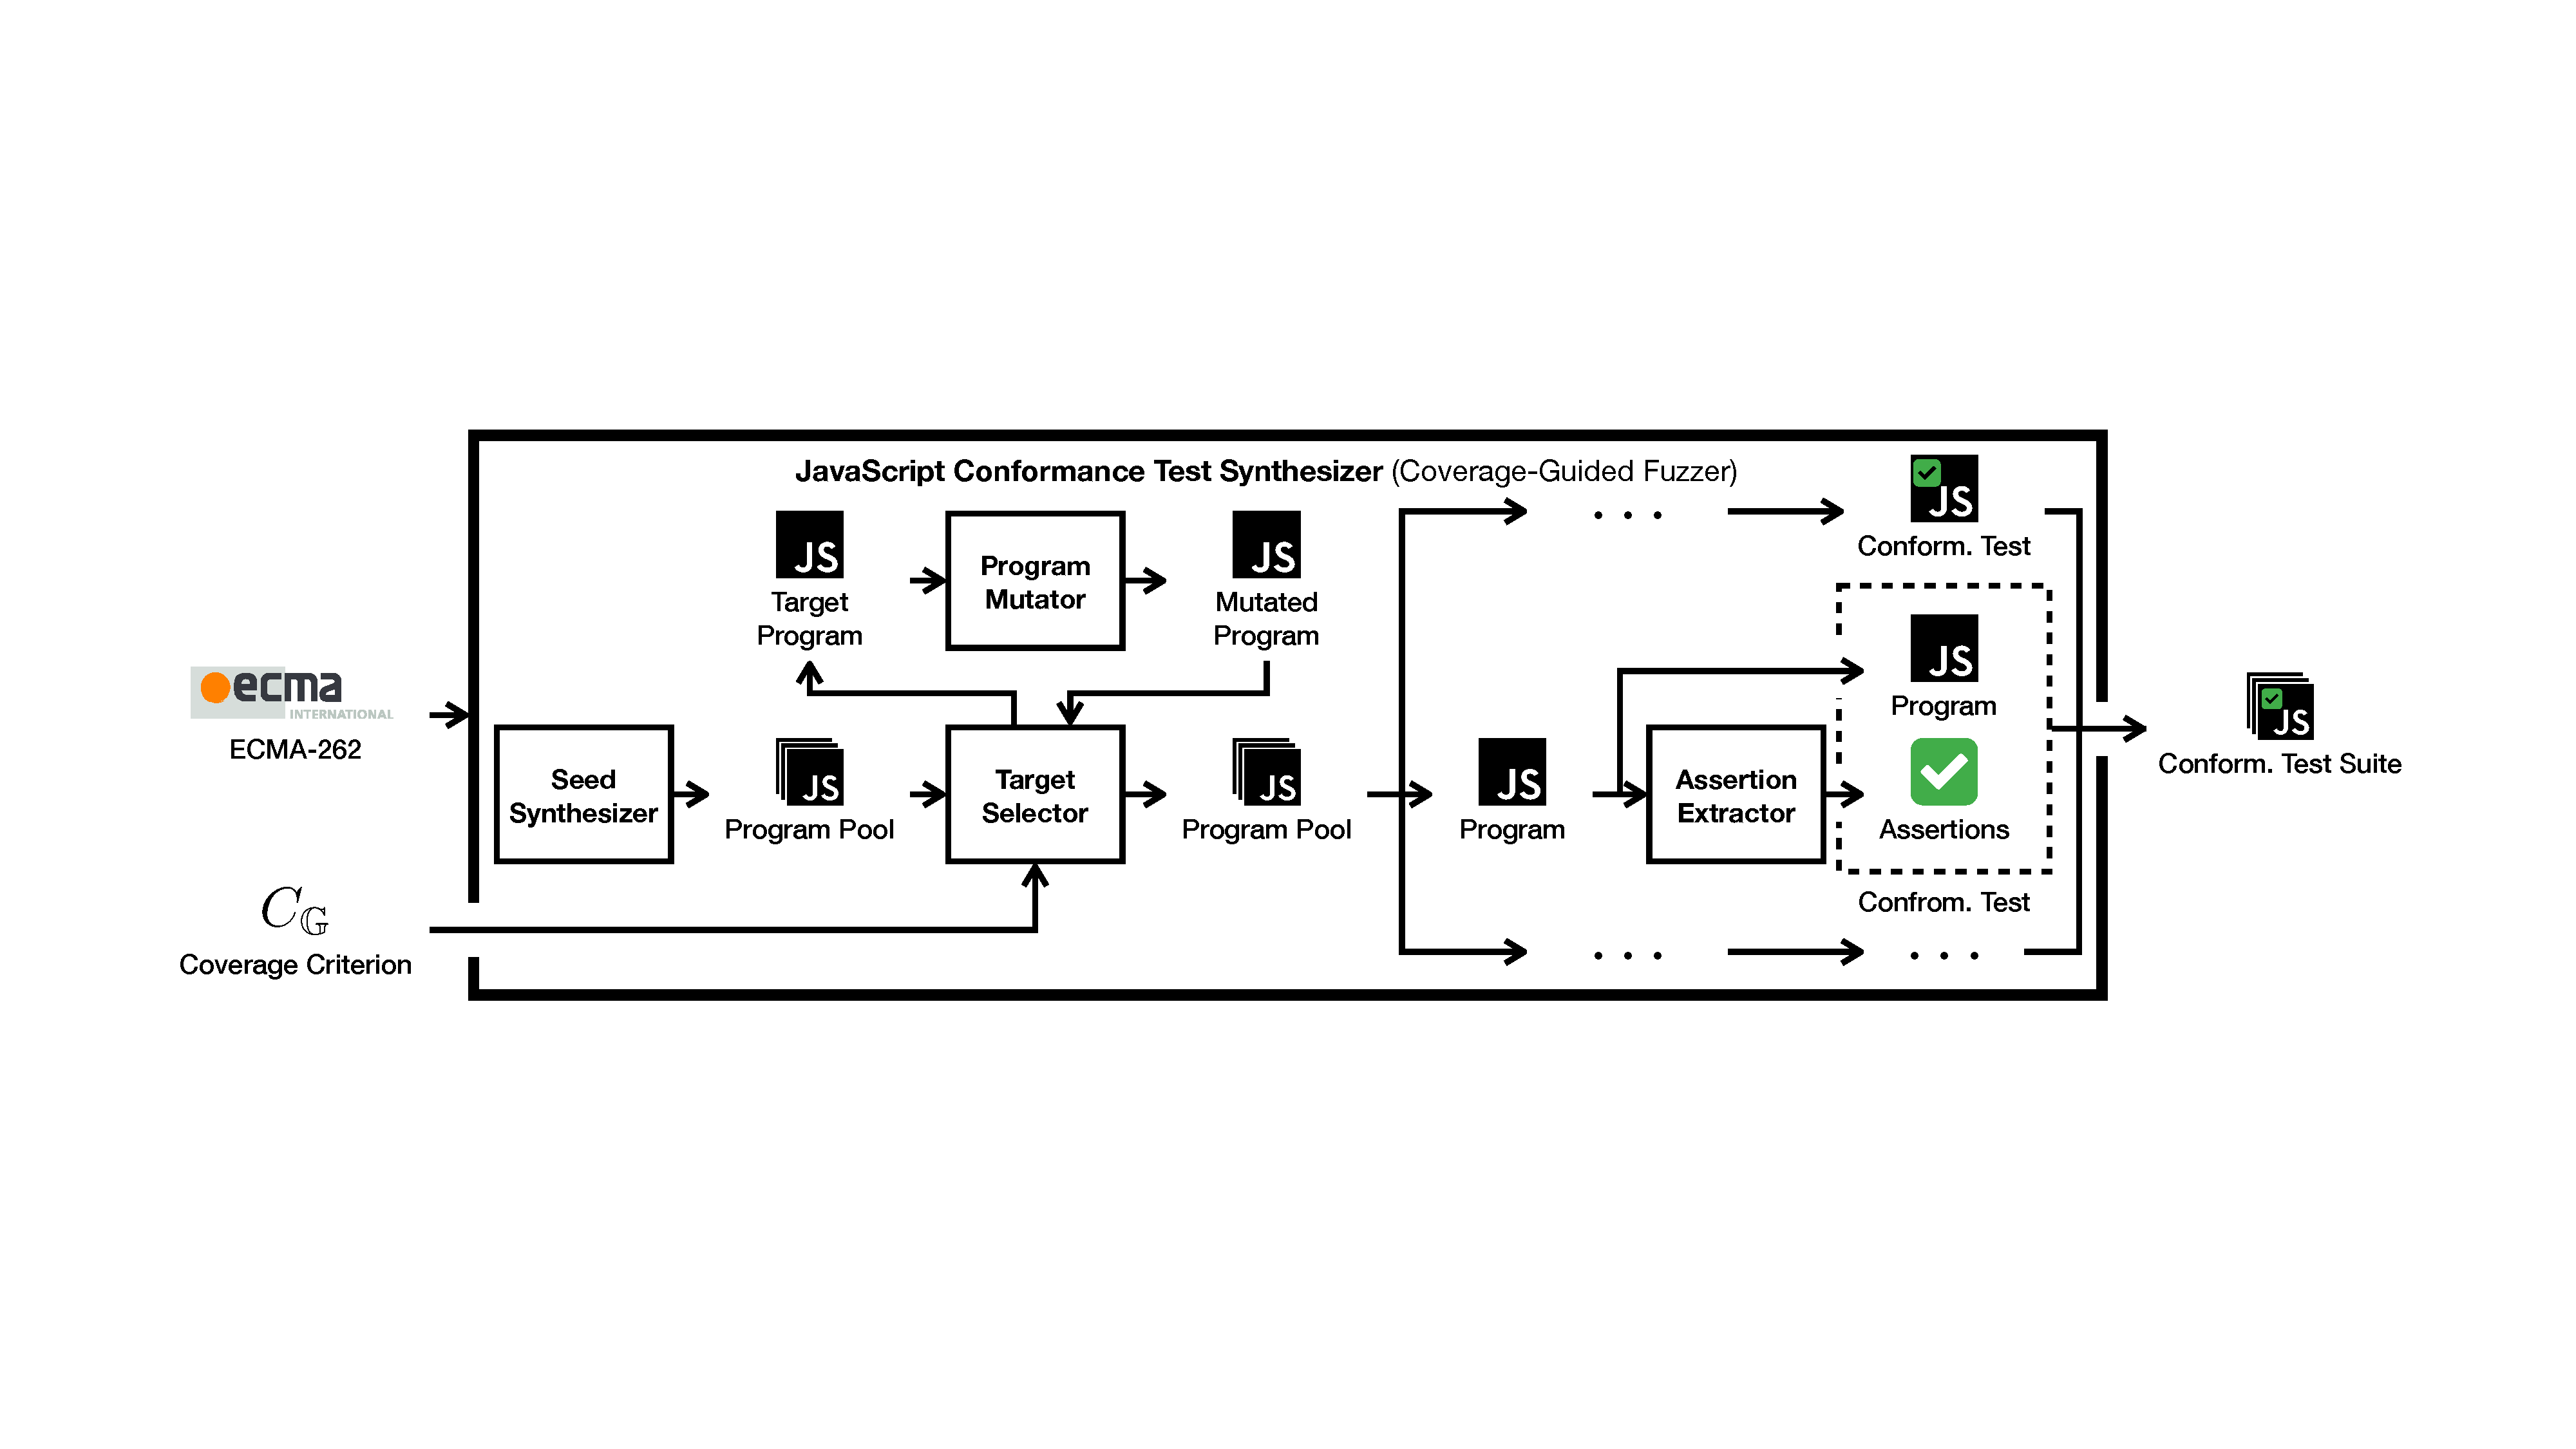
\includegraphics[width=\textwidth]{img/overall}
  \caption{
    Overall structure of a JavaScript conformance test synthesizer using
    coverage-guided fuzzing using the CFG of a mechanized specification
    extracted from the language specification, ECMA-262.
  }
  \label{fig:overall}
\end{figure}

%----------------------------------------%

First, we describe the overall structure of $\tool$ and explain which parts are
updated compared to the baseline tool.
%
$\jest$ is a state-of-the-art JavaScript conformance synthesizer using
coverage-guided fuzzing~\cite{afl} using the CFG in the language specification.
%
It utilizes another tool $\jiset$~\cite{jiset} to automatically extract a
mechanized specification directly from a given version of ECMA-262.
%
We extend $\jest$ to support both $k$-FS and $k$-FCPS coverage criteria.
%
Note that $\jest$ is recently updated based on $\esmeta$, a re-branded version
of $\jiset$ becuase it is deprecated now.\footnote{
  See \url{https://github.com/es-meta/esmeta}
}
%
As depicted in Figure~\ref{fig:overall}, it takes 1) the mechanized
specification for JavaScript, and 2) a coverage criterion $\cov{\graph}$ for CFG
of the specification.
%
We mark the extended part compared to the baseline as red to highlight.

$\tool$ consists of four modules that mechanically utilize JavaScript syntax and
semantics described in the given language specification.
\begin{itemize}
  \item \textsf{\textbf{Seed Synthesizer}}:
    %
    As the first step, \textsf{Seed Synthesizer} automatically synthesizes a set
    of JavaScript programs as the initial \textit{program pool}.
    %
    It utilizes JavaScript syntax described in the language specification to
    cover diverse alternatives in syntactic productions as much as possible.
    %
    Our tool uses existing two synthesizers: 1) a non-recursive synthesizer and
    2) a built-in synthesizer.
    %
  \item \textsf{\textbf{Target Selector}}:
    %
    To measure the coverage in the CFG, \textsf{Target Selector} extracts the
    execution path of each program in the pool by interpreting it using the
    abstract algorithms in the specification.
    %
    While the baseline tool supports only a node-or-branch coverage criterion,
    we extend it to support $k$-FS and $k$-FCPS node-or-branch coverage
    criteria as well.
    %
    If a program does not cover new TRs, it removes the program from the pool.
    %
    Then, it selects a program as a mutation target in the pool that potentially
    increases the coverage or stops the iteration when the current status
    satisfies the termination condition.
    %
  \item \textsf{\textbf{Program Mutator}}:
    %
    To increase the coverage in the CFG, \textsf{Program Mutator} repeatedly
    tries to mutate a JavaScript program to a new one based on mutation methods.
    %
    Our tool uses five existing mutation methods: 1) a random mutation, 2)
    nearest syntax tree mutation, 3) string substitution, 4) object
    substitution, and 5) statement insertion.
    %
  \item \textsf{\textbf{Assertion Extractor}}:
    %
    After the mutation iteration, \textsf{Assertion Extractor} automatically
    extracts seven kinds of assertions from each program in the pool.
    %
    The assertions represent the expected final state of each program according
    to the semantics described in the specification.
    %
    As a result, each pair of a program and the corresponding extracted
    assertions is a \textit{conformance test} for JavaScript.
\end{itemize}

%----------------------------------------%

\begin{figure}
  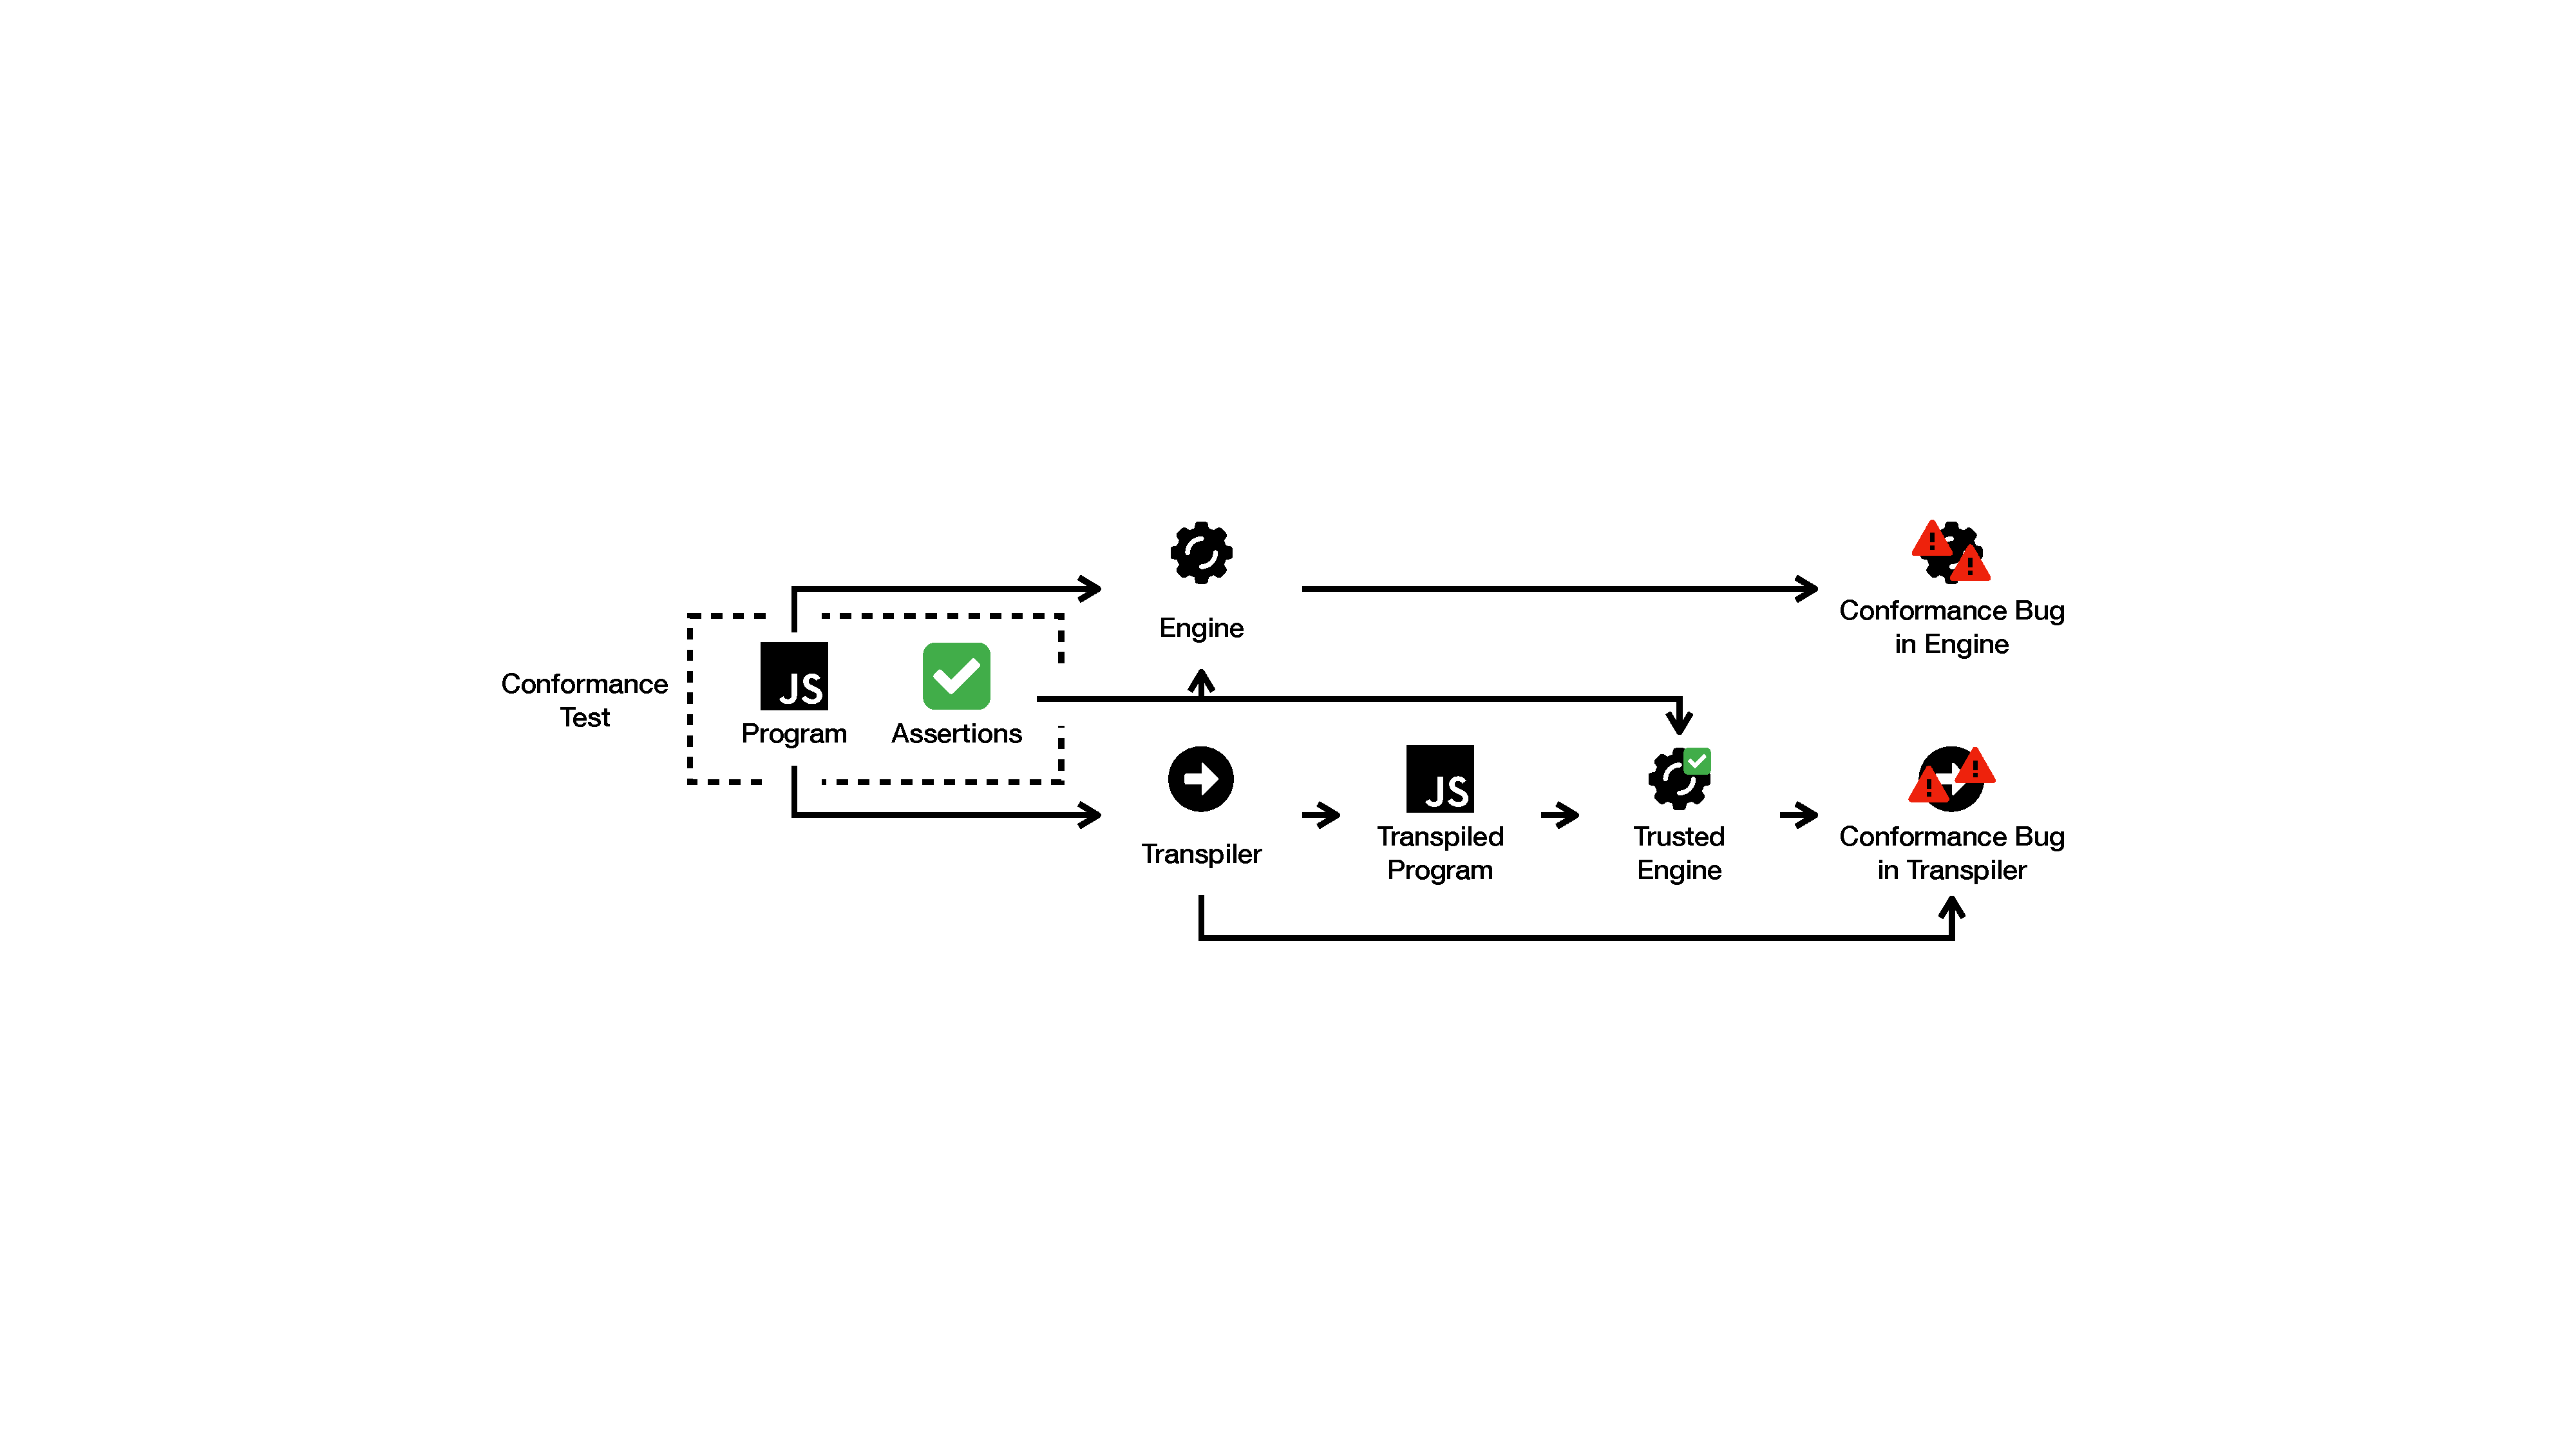
\includegraphics[width=\textwidth]{img/conform-check}
  \caption{
    Conformance check of both engines and transpilers with synthesized
    conformance tests.
  }
  \label{fig:conform-check}
\end{figure}

%----------------------------------------%
%----------------------------------------%

\paragraph{\textbf{Conformance Check of Engines and Transpilers}}
%
A synthesized conformance test consists of a JavaScript program and
corresponding assertions.
%
Figure~\ref{fig:conform-check} depicts how to use it to check the conformance of
JavaScript engines and transpilers.
%
First, assume that we want to check the conformance of a JavaScript engine.
%
In this case, it is enough to run the program and assertions together in the
target engine.
%
Then, if at least one assertion fails, we know the target engine has a
conformance bug related to the test.

On the other hand, we should transpile the program in the test for JavaScript
transpilers.
%
If the target transpiler abnormally terminates, it is a conformance bug because
the program of each conformance test is valid.
%
Otherwise, we should run the transpiled program and assertions together using an
engine.
%
Note that a trusted or already tested JavaScript engine is required to check the
conformance of the transpiler correctly.
%
Like the engine conformance check, the target transpiler has a conformance bug
related to the test if at least one assertion fails.

\begin{table}
\caption{
  Detected conformance bugs in JavaScript engines and transpilers
}
\vspace*{-.5em}
{
\footnotesize
\label{tab:conform-bugs}
\begin{tabular}{c?l|l|l?r|r|r}
\toprule\\[-1.6em]

\multicolumn{1}{c}{\multirow{2}{*}{\textbf{Kind}}}
& \multicolumn{1}{c|}{\multirow{2}{*}{\textbf{Name}}}
& \multicolumn{1}{c|}{\multirow{2}{*}{\textbf{Version}}}
& \multicolumn{1}{c?}{\multirow{2}{*}{\textbf{Release}}}
& \multicolumn{3}{c}{\textbf{\# Detected Unique Bugs}} \\\cline{5-7}

&&&
& \multicolumn{1}{c|}{\textbf{\# New}}
& \multicolumn{1}{c|}{\textbf{\# Confirmed}}
& \multicolumn{1}{c}{\textbf{\# Reported}}\\

\toprule\\[-1.6em]

\multirow{5}{*}{Engine}
& V8            & v10.8.121 & 2022.10.06 & 0 & 0 & 4 \\\cline{2-7}
& JSC           & v615.1.10 & 2022.10.26 & 15 & 15 & 24\\\cline{2-7}
& GraalJS       & v22.2.0   & 2022.07.26 & 9 & 9 & 10 \\\cline{2-7}
& SpiderMonkey  & v107.0b4  & 2022.10.24 & 1 & 3 & 4 \\\cline{2-7}
& \multicolumn{3}{c?}{\textbf{Total}}    & \textbf{25}& \textbf{27}& \textbf{42}\\

\toprule\\[-1.6em]

\multirow{5}{*}{Transpiler}
& Babel         & v7.19.1   & 2022.09.15 & 30& 30& 35\\\cline{2-7}
& SWC           & v1.3.10   & 2022.10.21 & 27& 27& 41\\\cline{2-7}
& Terser        & v5.15.1   & 2022.10.05 & 1 & 1 & 18\\\cline{2-7}
& Obfuscator    & v4.0.0    & 2022.02.15 & 0 & 0 & 7 \\\cline{2-7}
& \multicolumn{3}{c?}{\textbf{Total}}    & \textbf{58}& \textbf{58}& \textbf{101}\\

\toprule\multicolumn{1}{c}{}\\[-1.6em]


\multicolumn{4}{c?}{\textbf{Total}}
& \textbf{83}& \textbf{85}& \textbf{143}\\

\toprule\multicolumn{1}{c}{}\\[-1.6em]
\end{tabular}
}
\end{table}

\section{Evaluation}\label{sec:eval}
This section evaluates feature-sensitive coverage criteria with the following research questions:
\begin{itemize}
  \item \textbf{RQ1 (Conformance Bug Detection):} How many conformance bugs
 in JavaScript implementations are detected by synthesized conformance tests?
    (Section~\ref{sec:conform-bug})
  \item \textbf{RQ2 (Effectiveness of $k$-FS Coverage Criteria):} Are higher $k$-FS
    coverage criteria more effective than lower $k$-FS coverage
    criteria in detecting conformance bugs? (Section~\ref{sec:impact-k-fs})
  \item \textbf{RQ3 (Effectiveness of $k$-FCPS Coverage Criteria):} Are $k$-FCPS
    coverage criteria more effective than $k$-FS coverage criteria in detecting
    conformance bugs? (Section~\ref{sec:impact-k-fcps})
  \item \textbf{RQ4 (Comparison with Test262):} Can conformance tests
    synthesized by $\tool$ complement Test262, the official JavaScript conformance
    suite maintained manually? (Section~\ref{sec:compare-test262})
\end{itemize}

We apply $\tool$ to the latest language specification (ES13, 2022)~\cite{es13},
which synthesized 237,981 conformance tests in 50 hours with
five graph coverage criteria: 1) 0-FS, 2) 1-FS, 3) 2-FS, 4) 1-FCPS,
and 5) 2-FCPS node-or-branch coverage.
We performed our experiments with five Ubuntu machines with a 4.0GHz Intel(R)
Core(TM) i7-6700k and 32GB of RAM (Samsung DDR4 2133MHz 8GB*4).

%----------------------------------------%

Using the synthesized JavaScript conformance tests, we check the conformance of
eight mainstream implementations listed in Table~\ref{tab:conform-bugs}.
We select them as evaluation targets because they support all the language
features in ES13.
V8, JSC, and SpiderMonkey are JavaScript engines used in web browsers, Google
Chrome, Apple Safari, and Mozilla Firefox, respectively, and
GraalJS is a JavaScript engine by Oracle.
Babel and SWC are transpilers that desugar new language features into old ones,
usually ES5.1 features, for legacy host environments.
Terser is a code compressor that reduces code size, and
Obfuscator obfuscates code to make it hard to understand and reverse-engineering.
For the transpiler conformance check, we use V8 as the default engine
to execute transpiled code with assertions.
If a test fails on V8, we use another engine that passes the test;
if a test fails on all engines, we do not use the test.

%----------------------------------------%

%----------------------------------------%
%----------------------------------------%

\subsection{Conformance Bug Detection}\label{sec:conform-bug}

%----------------------------------------%

Table~\ref{tab:conform-bugs} summarizes the conformance bugs
detected by $\tool$ in all the evaluation targets.
We manually inspected the failed conformance test cases,
found 143 distinct conformance bugs, and reported them to
the corresponding developers.
%
As a result, 85 out of 143 bugs were officially confirmed, and
83 were newly discovered bugs.
%
The other 47 reported bugs are still under review, or developers have
not yet responded.
%
Among 143 detected bugs, 42 are engine bugs, and 101 are
transpiler bugs.
We present two real-world bug examples.

%----------------------------------------%

\paragraph{\textbf{Order of Execution}}
%
JavaScript engines must follow the execution order of each language feature
described in the language specification.
%
However, we found a bug\footnote{
  We anonymized links of bug reports for double-blinded reviewing.
  % TODO during camera-ready
  % https://github.com/oracle/graaljs/issues/655
  % https://github.com/oracle/graaljs/issues/671
} related to the execution order of the \jscode{delete} operation that causes
the execution of originally unreachable code in GraalJS.
%
For example, while the following code should return \jscode{false}, it throws an
exception with \jscode{"ERR"} by executing the originally unreachable code
inside the arrow function in GraalJS:
%
\begin{lstlisting}[style=JS, basicstyle=\footnotesize\ttfamily]
    false && delete (() => { throw "ERR"; })(); // Expected: false
\end{lstlisting}
%
In addition, we detected another bug\footnote{
  We anonymized links of bug reports for double-blinded reviewing.
  % TODO during camera-ready
  % V8 - https://bugs.chromium.org/p/v8/issues/detail?id=13469
  % GraalJS - https://github.com/oracle/graaljs/issues/673
  % JSC - https://bugs.webkit.org/show_bug.cgi?id=247723
  % SpiderMonkey - https://bugzilla.mozilla.org/show_bug.cgi?id=1800062
  % ECAM-262 - https://github.com/tc39/ecma262/issues/2659
} related to the execution order of property reads
%
% For example, while the following code should throw an exception with
% \jscode{"ERR"}, V8 throws a \textbf{TypeError} exception:
%
% \begin{lstlisting}[style=JS, basicstyle=\footnotesize\ttfamily]
% null [ { [Symbol.toPrimitive ] : () => { throw "ERR"; } } ];
% \end{lstlisting}
%
in all target engines. ECMA-262 may consider changing the semantics
according to the one used in most implementations.

%----------------------------------------%

\paragraph{\textbf{Asynchronous Function / Generator}}
One of the complex language features in JavaScript is asynchronous functions and
generators introduced in ES6 (2015).
%
We detected a bug\footnote{
  We anonymized links of bug reports for double-blinded reviewing.
  % TODO during camera-ready
  % https://github.com/tc39/proposal-async-await/issues/60
  % https://bugzilla.mozilla.org/show_bug.cgi?id=1799288
} in SpiderMonkey that breaks the logic of asynchronous function calls.
%
For example, the following code must return a rejected \jscode{Promise} object
because a non-iterable value \jscode{undefined} is assigned to an array
destructuring pattern \jscode{[]} in the \jscode{async} arrow function:
%
\begin{lstlisting}[style=JS, basicstyle=\footnotesize\ttfamily]
    (async function ([]) {})(); // Expected: A rejected Promise object
\end{lstlisting}
However, it unexpectedly terminates with a \textbf{TypeError} exception in SpiderMonkey.
A developer of SpiderMonkey explained it as follows:
\begin{quote}
``The \jscode{async}-function spec was changed at some point \textelp{}\\
this is also not covered by test262.''
\end{quote}
%
% We also detected other similar bugs related to generators in the SWC transpiler,
% and its main developer appreciated our work and requested us to apply our tool
% for SWC using the \scode{jsc.minify} option as well.\footnote{
%   We anonymized links of bug reports for double-blinded reviewing.
%   % TODO during camera-ready
%   % https://github.com/swc-project/swc/issues/6375
% }

%----------------------------------------%
% \paragraph{\textbf{JSC}}
% %
% For JSC, we detected a conformance bug related to the order of properties for
% \jscode{class} expressions.
% % https://bugs.webkit.org/show_bug.cgi?id=247429
% In the following code, the variable \jscode{order} should be an array
% \jscode{["length", "name", "prototype"]}:
% \begin{lstlisting}[style=JS, basicstyle=\footnotesize\ttfamily]
% class C { static D = class {}; } let order = Reflect.ownKeys(C.D);
% \end{lstlisting}
% %
% However, it becomes \jscode{["length", "prototype", "name"]} in JSC.
% %
% This conformance bug is a hard-to-find bug because it is reproducible only when
% a \jscode{class} expression is assigned to a static field of another
% \jscode{class} declaration or expression.

%----------------------------------------%

% %
% Based on our bug reports, the developers of the Babel transpiler realilzed that
% Babel have many \textit{temporal dead zone (TDZ)} bugs caused by \jscode{let} or
% \jscode{const}.
% % https://github.com/babel/babel/issues/15150
% % (EXAMPLE) let x = x;
% % (EXAMPLE with TDZ option) const x = 0; x = 1;
% Thus, they created a special label \name{Spec: TDZ} to highlight issues related
% to TDZ bugs and started to fix bugs related to TDZ bugs.

%----------------------------------------%
%----------------------------------------%

\subsection{Effectiveness of $k$-FS Coverage Criteria}\label{sec:impact-k-fs}

\begin{table}
\caption{
  Comparison of synthesized conformance tests guided by five graph coverage criteria
}
\vspace*{-.5em}
{
\footnotesize
\label{tab:compare}
\begin{tabular}{c?r|r|r?r|r}
\toprule\\[-1.6em]

\multicolumn{1}{c}{\multirow{2}{*}{\textbf{Coverage Criteria} $\cov{\graph}$}}
& \multicolumn{3}{c?}{\textbf{\# Covered $k$-F(CP)S-TR (k)}}
& \multicolumn{1}{c|}{\multirow{2}{*}{\textbf{\# Syn. Test}}}
& \multicolumn{1}{c}{\multirow{2}{*}{\textbf{\# Bug}}}\\\cline{2-4}

& \multicolumn{1}{c|}{\textbf{\# Node}}
& \multicolumn{1}{c|}{\textbf{\# Branch}}
& \multicolumn{1}{c?}{\textbf{\# Total}}
&&\\

\toprule\\[-1.6em]

0-FS node-or-branch (\sname{0-fs})
& 10.0    & 5.6     & 15.6    & 2,111  & 55  \\\hline
1-FS node-or-branch (\sname{1-fs})
& 79.3    & 45.7    & 125.0   & 6,766  & 83  \\\hline
2-FS node-or-branch (\sname{2-fs})
& 1,199.8 & 696.3   & 1,896.1 & 97,423 & 102 \\\hline
1-FCPS node-or-branch (\sname{1-fcps})
& 179.7   & 97.6    & 277.3   & 9,092  & 87  \\\hline
2-FCPS node-or-branch (\sname{2-fcps})
& 2,323.1 & 1,297.6 & 3,620.7 & 122,589& 111 \\

\toprule\multicolumn{1}{c}{}\\[-1.6em]

\end{tabular}
}
\end{table}

%----------------------------------------%

Table~\ref{tab:compare} shows the result of conformance test synthesis via
$\tool$ with five graph coverage criteria.
%
Note that 0-FS node-or-branch coverage criterion is the same with the node-or-branch
coverage criterion.
%
To evaluate the effectiveness of $k$-FS coverage criteria, we compare the synthesized
conformance tests guided by different $k$-FS node-or-branch coverage criteria
(\sname{0-fs}, \sname{1-fs}, and \sname{2-fs} in Table~\ref{tab:compare}).
%
The second to the fourth columns denote the numbers of covered $k$-FS- or $k$-FCPS-TRs for
nodes (\textbf{\small \# Node}), branches (\textbf{\small \# Branch}), and both
(\textbf{\small \# Total}), respectively.
%
The fifth and the sixth columns denote the numbers of synthesized conformance tests
(\textbf{\small\# Syn. Test}) and detected distinct bugs
(\textbf{\small\# Bug}), respectively.

%----------------------------------------%

The results show that higher $k$-FS coverage criteria are more
effective than lower $k$-FS.
On average, 8.03 (125.0K / 15.6K) 1-FS-TRs exist per each 0-FS-TR, and 15.17 (1,896.1K
/ 125.0K) 2-FS-TRs exist per each 1-FS-TR.
%
It means that each node or branch is used in 8.03 different language features,
and each language feature could be used in 15.17 other language features on average.
%
For a more detailed information, we draw a histogram of the number of covered
1-FS-TRs (or 2-FS-TRs) per each covered 0-FS-TR (or 1-FS-TR) in
Figures~\ref{fig:hist} (a) and (b).
%
The largest number of covered 1-FS-TRs per each covered 0-FS-TR is 303
for a node in the \textbf{[[GetOwnProperty]]} algorithm.
%
In other words, this algorithm is used in 303 different language features,
because the semantics of many syntactic or built-in API features use
this algorithm to access object properties.
%
The largest number of covered 2-FS-TRs per each covered 1-FS-TR is 116
for a node whose innermost enclosing feature is the syntactic feature $\idfeat$
for identifier references explained in Section~\ref{sec:fcps-cov}.
%
In other words, the syntactic feature $\idfeat$ is used in 116 different
language features, because identifier references can be used in
diverse syntactic features, such as function names, destructuring
patterns, and property definitions.
%
The number of synthesized tests increased 3.21x (6,766 / 2,111) from 0-FS to
1-FS coverage criteria and 14.4x (97,423 / 6,766) from 1-FS to 2-FS coverage
criteria.
%
In addition, the number of detected unique bugs also increased when using higher
$k$-FS node-or-branch coverage criteria.
%
The baseline with 0-FS coverage criterion detects 55 conformance bugs in engines
and transpilers.
%
The conformance tests synthesized with 1-FS coverage criterion detect 28
(83 - 55) more conformance bugs, and tests synthesized with 2-FS coverage
criterion detect 4 (87 - 83) more bugs.
%
Now, we present two bug examples that show the effectiveness of $k$-FS coverage
criteria.

%----------------------------------------%

\paragraph{\textbf{Empty Name Binding for \jscode{let} in \jscode{for}-Loop}}
%
JavaScript provides diverse shapes of $\jscode{for}$-loops as syntactic features
defined with the \esnt{ForStatement} production.
%
Among them, a \jscode{for}-loop with a \jscode{let}-binding is
its third alternative.
%
While it normally has one or more name bindings, we can pass an empty list of
name bindings using an empty object destructuring pattern \jscode{\{\}}.
%
However, Babel crashes when transpiling a \jscode{for}-loop with
empty name bindings for \jscode{let}:\footnote{
  We anonymized links of bug reports for double-blinded reviewing.
  % TODO during camera-ready
  % https://github.com/babel/babel/issues/15100
}
%
\begin{lstlisting}[style=JS, basicstyle=\footnotesize\ttfamily]
    for (let {} = 0; 0; ) ; // Expected: Normally terminates
\end{lstlisting}
%
Because the \textbf{CreatePerIterationEnvironment} algorithm that checks
the empty name bindings is used for other language features,
the tests synthesized with a 0-FS coverage criterion
failed to detect this conformance bug.
On the other hand, feature-sensitive coverage criteria can discriminate the
usage of the empty name binding checking semantics in different language features.
Thus, we successfully detected this conformance bug with 1-FS, 2-FS,
1-FCPS, and 2-FCPS coverage criteria.

%----------------------------------------%

\paragraph{\textbf{Computed Property for \jscode {async} Method in
\jscode{class}}}
%
JavaScript provides \textit{computed properties} to
allow defining property names using any expressions.
%
For example, let's define an object using a computed property: \jscode{let x =
\{ ["a" +"b" ]() \{ return 42 \} \}}.
%
Then, \jscode{x} is an object having a property \jscode{ab} that stores a
function as a method of the object: \jscode{x.ab() === 42}.
%
In addition, it also assigns the \jscode{name} property of the function as the
property name: \jscode{x.ab.name === "ab"}.
%
However, JSC does not follow this semantics when the computed property
is used for an \jscode{async} method inside classes.
%
For example, the following program checks whether the \jscode{name} property of
the \jscode{async} method in the class \jscode{C} is \jscode{"f"}:\footnote{
  We anonymized links of bug reports for double-blinded reviewing.
  % TODO during camera-ready
  % https://github.com/babel/babel/issues/15100
}
%
\begin{lstlisting}[style=JS, basicstyle=\footnotesize\ttfamily]
    class C { async ["f"] () {} } // Expected: C.prototype.f.name === "f"
\end{lstlisting}
%
However, the \jscode{name} property is \jscode{"async"} instead of \jscode{"f"}
in the JSC engine.
%
Since it is a combination of a \jscode{class}, an \jscode{async} method, and a
computed property, 0 or 1-FS coverage criteria may not keep it in the final
program pool.
On the other hand, 2-FS coverage criterion can discriminate it with other tests.
%
If a conformance test covers 2-FS-TR consisting of two syntactic features
\esnt{AsyncMethod} production with \textbf{PropMethod} SDO and
\esnt{ComputedProeprtyName} production with \textbf{PropMethod} SDO,
it can find this conformance bug.
Our experiment successfully detected this conformance bug with tests synthesized
with 2-FS and 2-FCPS coverage criteria.

%----------------------------------------%
%----------------------------------------%

\subsection{Effectiveness of $k$-FCPS Coverage Criteria}\label{sec:impact-k-fcps}

\begin{figure}
  \centering
  \begin{subfigure}{0.24\textwidth}
    \centering
    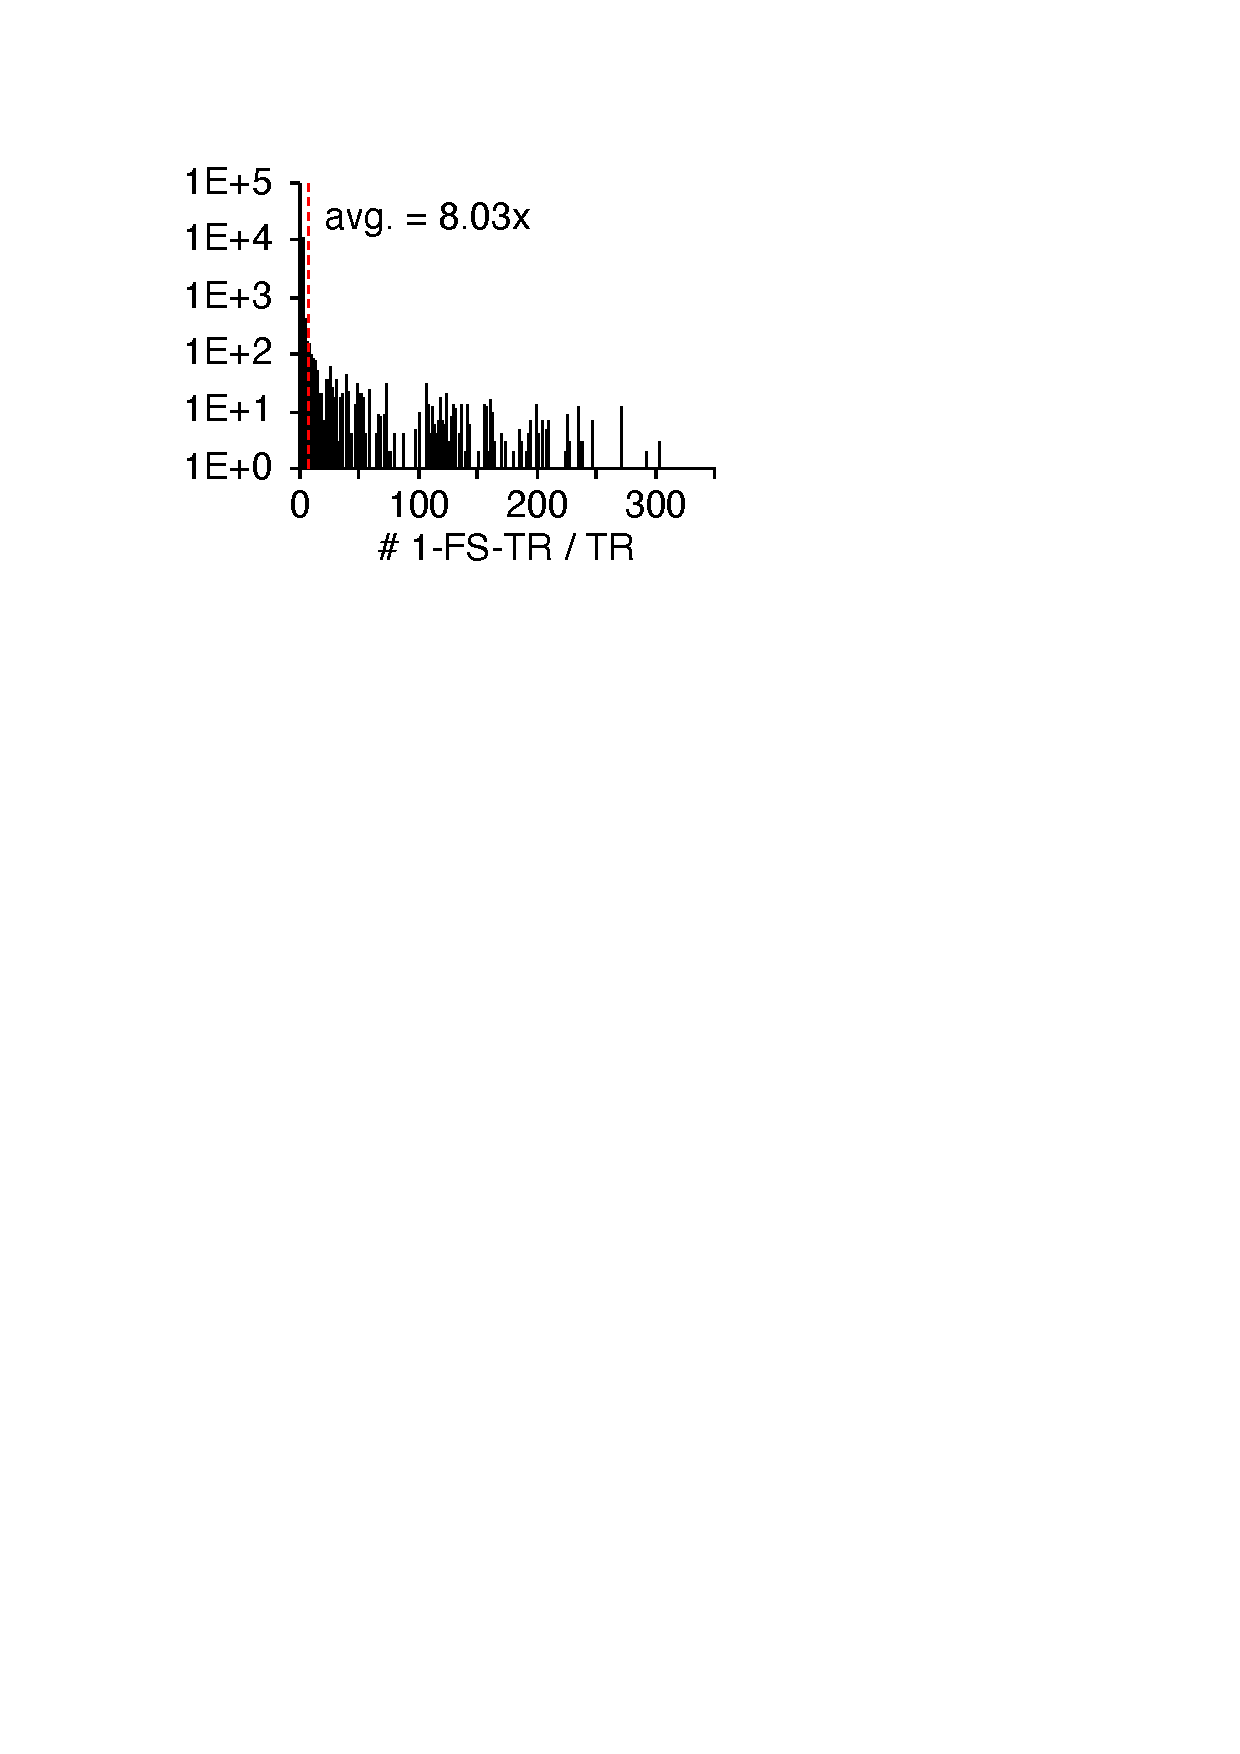
\includegraphics[width=\textwidth]{img/1-fs-hist}
    \subcaption{1-FS-TRs vs base TR}
  \end{subfigure}
  \begin{subfigure}{0.24\textwidth}
    \centering
    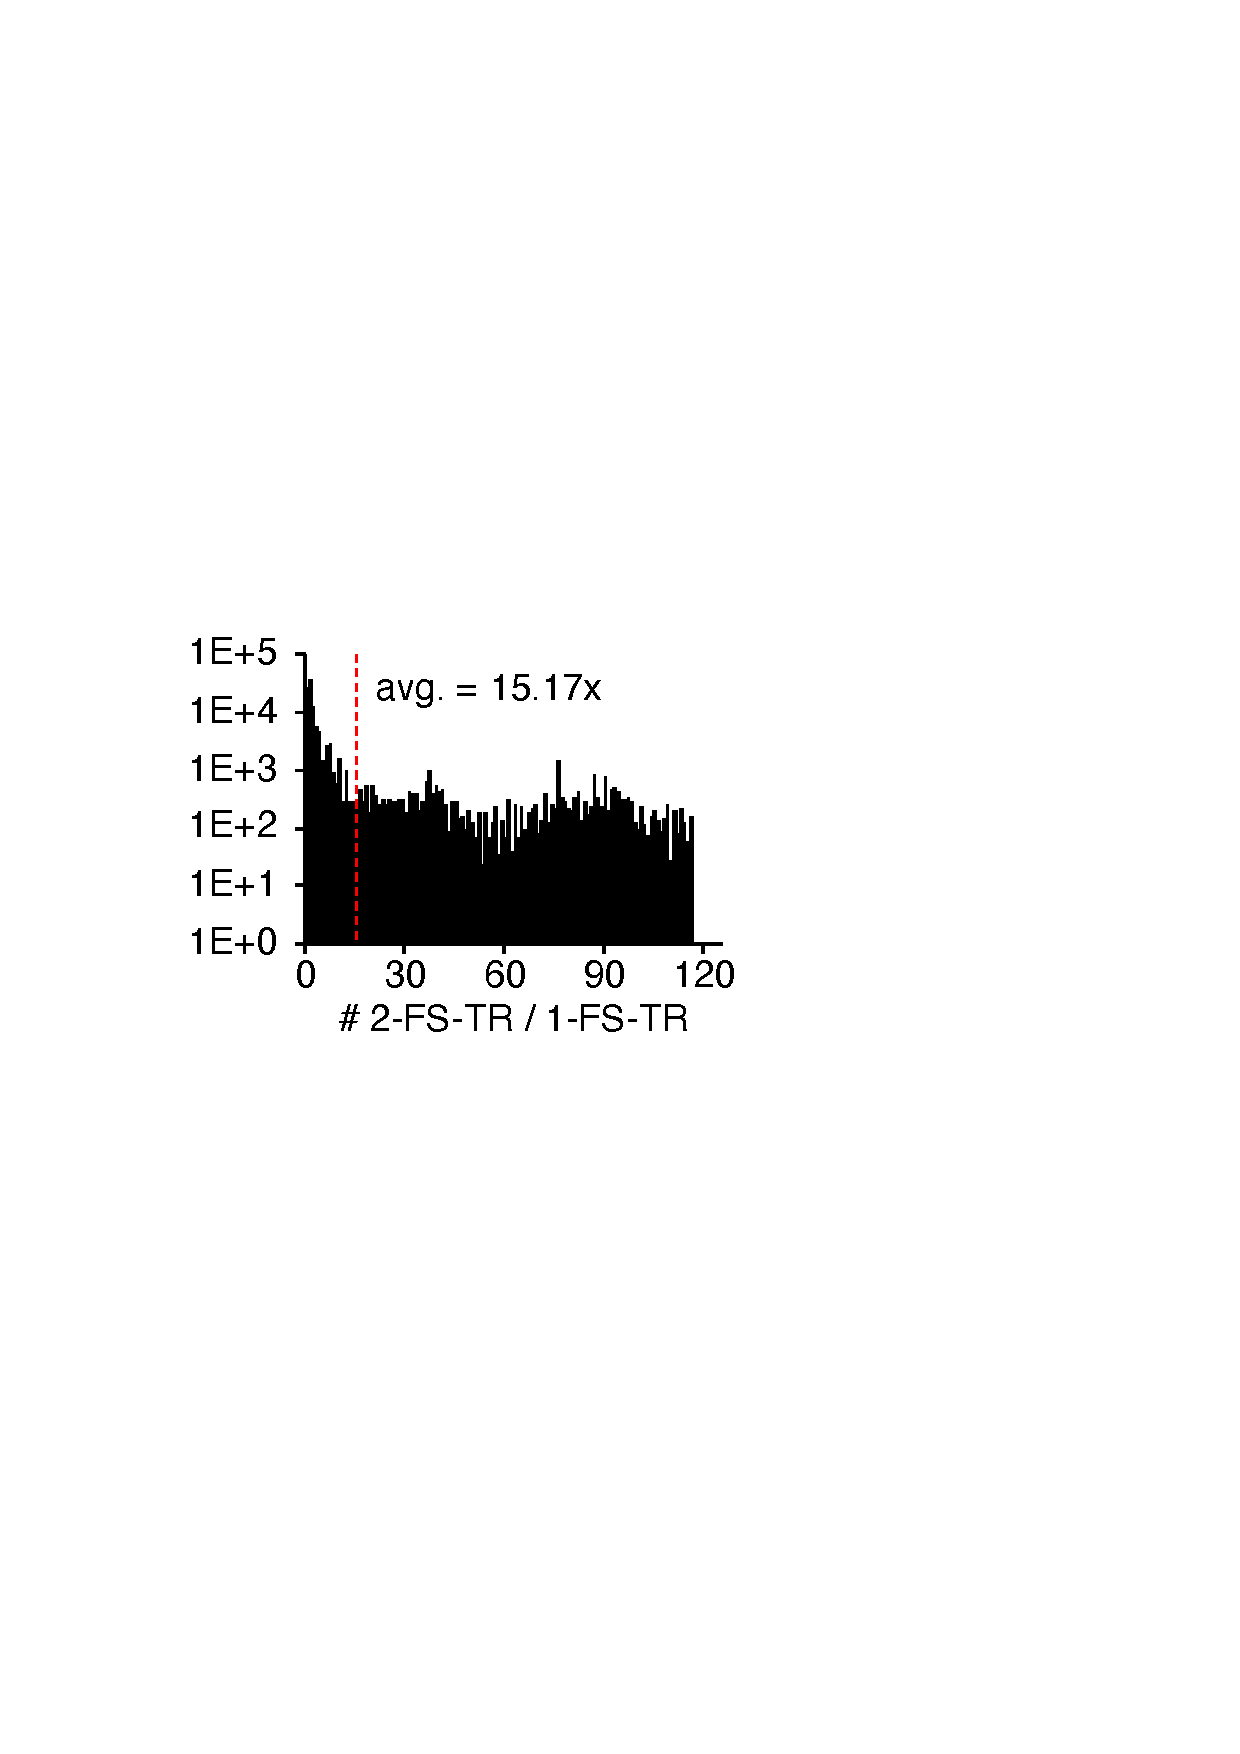
\includegraphics[width=\textwidth]{img/2-fs-hist}
    \subcaption{2-FS-TRs vs 1-FS-TR}
  \end{subfigure}
  \begin{subfigure}{0.24\textwidth}
    \centering
    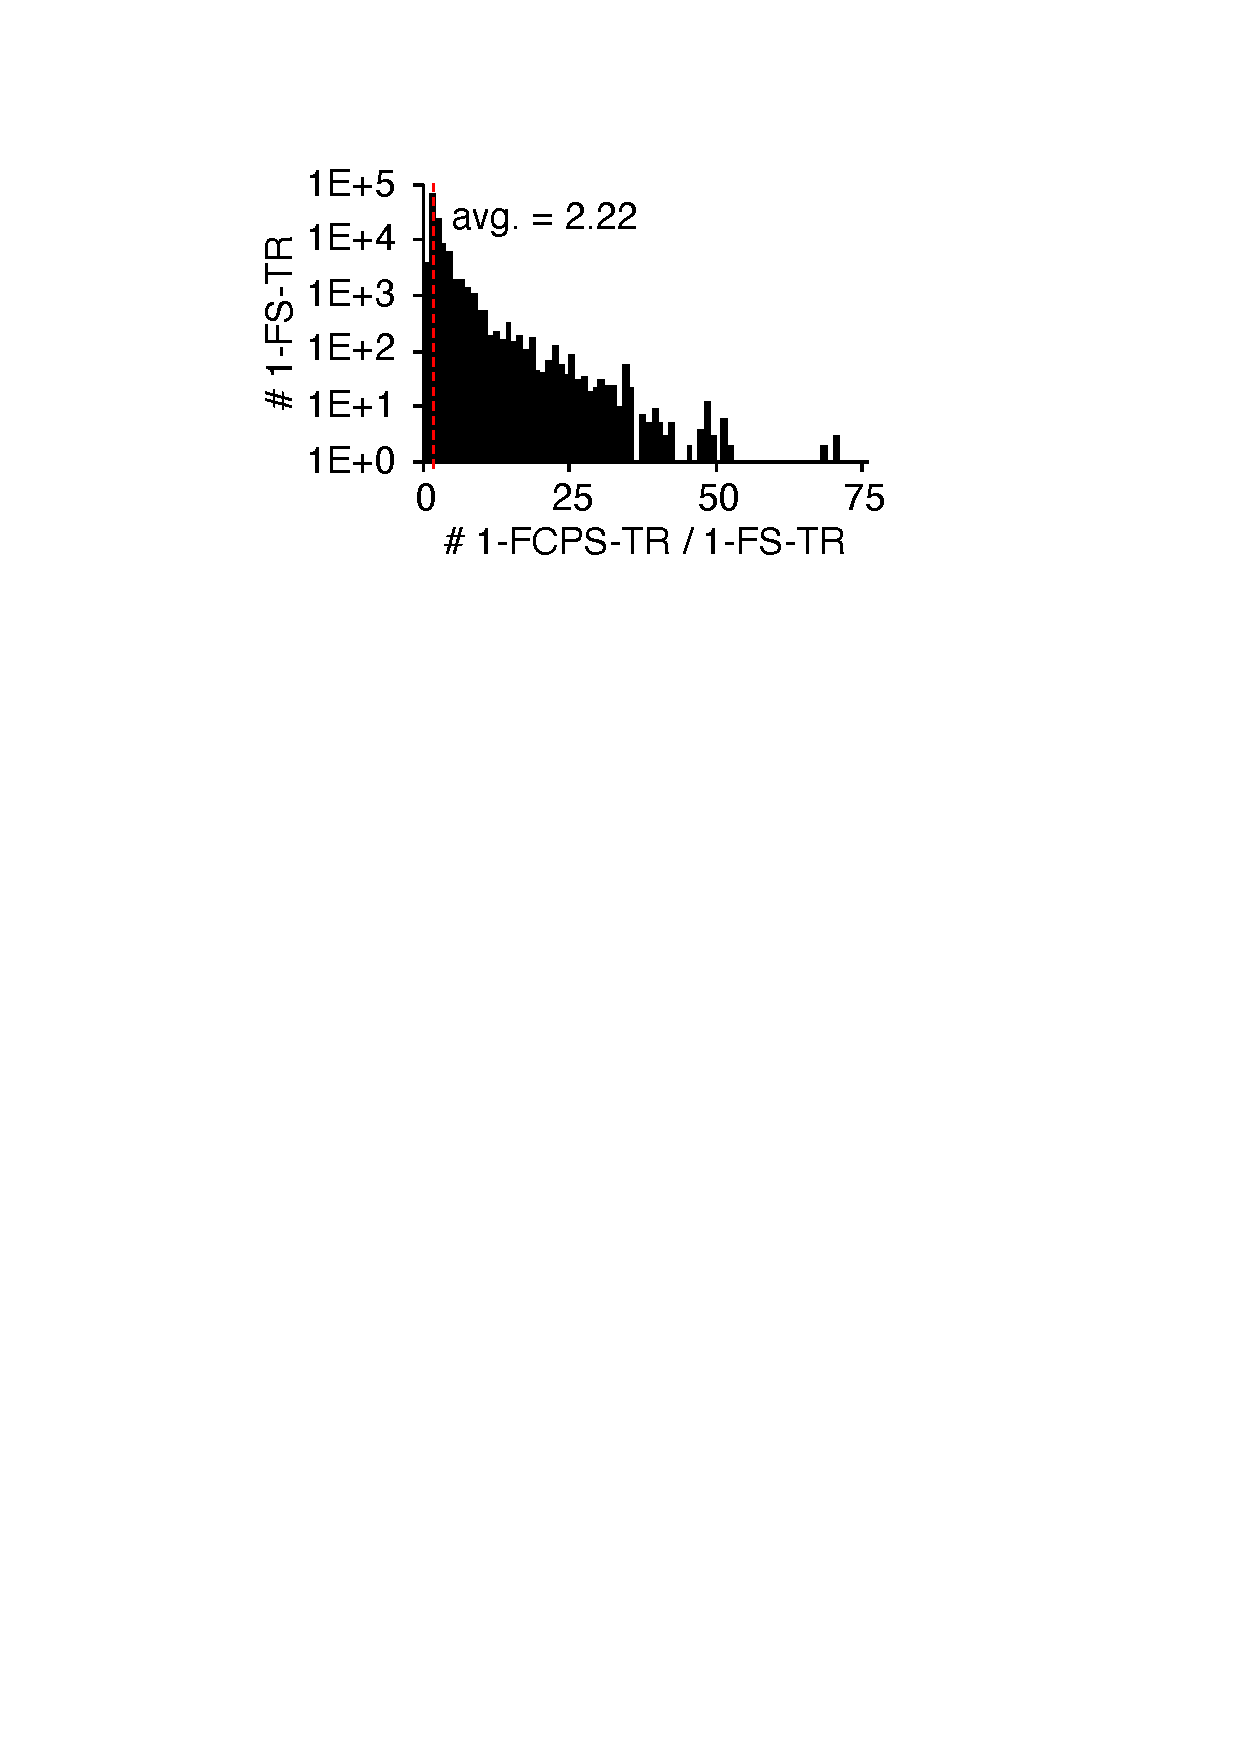
\includegraphics[width=\textwidth]{img/1-fcps-hist}
    \subcaption{1-FCPS-TRs vs 1-FS-TR}
  \end{subfigure}
  \begin{subfigure}{0.24\textwidth}
    \centering
    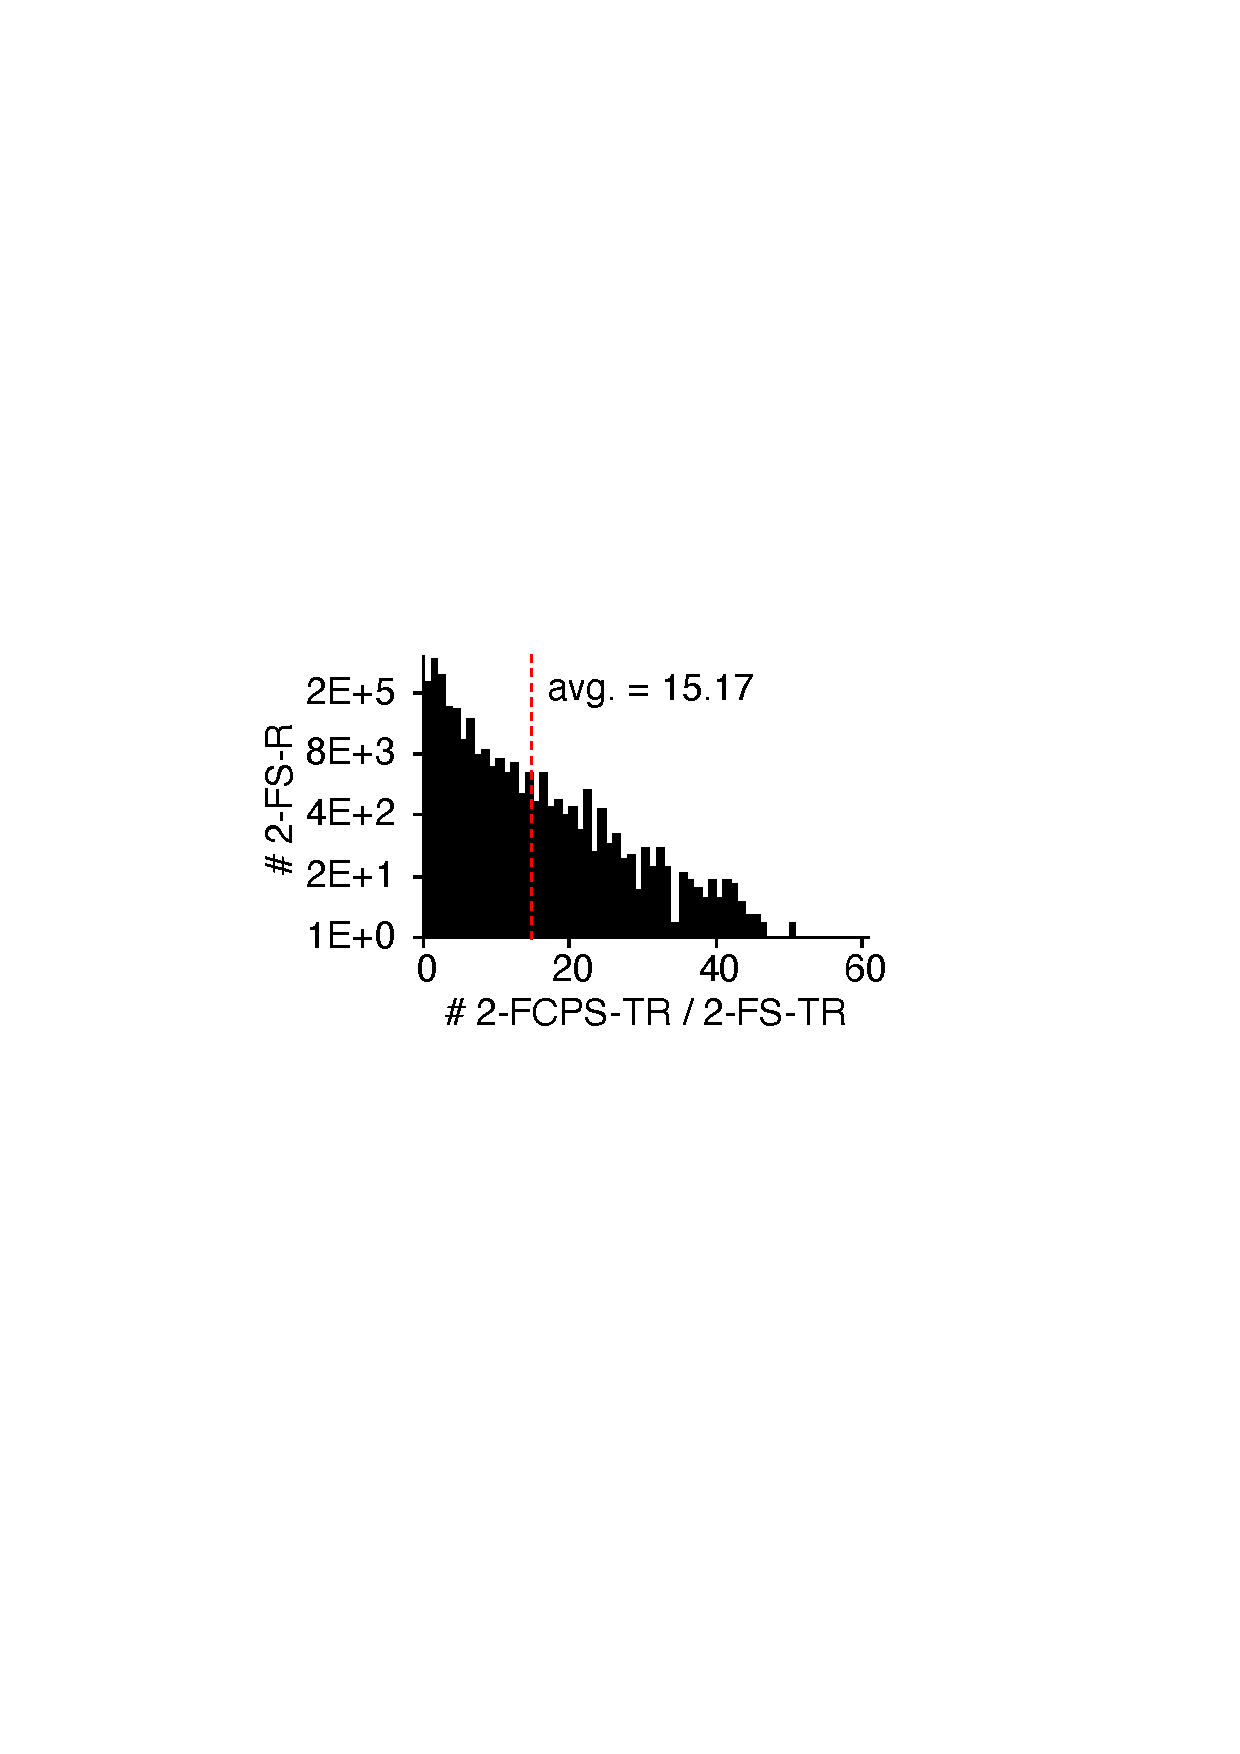
\includegraphics[width=\textwidth]{img/2-fcps-hist}
    \subcaption{2-FCPS-TRs vs 2-FS-TR}
  \end{subfigure}
  \caption{
    The histogram of numbers of $k$-FS or $k$-FCPS TRs per less sensitive $k$-FS
    or $k$-FCPS TR
  }
  \label{fig:hist}
\end{figure}

%----------------------------------------%

We also evaluate the effectiveness of $k$-FCPS coverage criteria compared to $k$-FS
coverage criteria.
%
According to Table~\ref{tab:compare}, the number of covered 1-FCPS- and
2-FCPS-TRs are 277.3K and 3,620.7K, respectively.
%
Thus, 2.22 (277.3K / 125.0K) 1-FCPS-TRs exist per each 1-FS-TR, and 1.91
(3,620.7K / 1,896.1K) 2-FCPS-TRs exist per each 2-FS-TR on average.
%
It means that 2.22 and 1.91 feature-call-paths exist from the innermost
language features to nodes or branches in each 1-FS-TR and 2-FS-TR,
respectively.
%
For a more detailed information, we also draw a histogram of the number of
covered 1-FCPS-TRs (or 2-FCPS-TRs) per each covered 1-FS-TR (or 2-FS-TR) in
Figures~\ref{fig:hist} (c) and (d).
%
The largest number of covered 1-FCPS-TRs per 1-FS-TR is 70 for a node
in the \jscode{Array.prototype.splice} built-in method.
%
It is a powerful built-in API feature that changes the contents of an array by
removing or replacing existing elements and/or adding new elements in place.
%
Thus, its semantics is quite complex and uses diverse helper functions, and the
number of possible feature-call-paths in this featuere is much larger than
the others.
%
The largest number of 2-FCPS-TRs per 2-FS-TR is 53 for a node whose
innermost enclosing feature is a syntactic feature for \jscode{yield} expressions
because it touches various helper functions for asynchronous behaviors.
%
Because of the increased number of TRs, the number of synthesized tests also
increased 1.34x (9,092 / 6,766) from 1-FS to 1-FCPS coverage criteria and 1.26x
(122,589 / 97,423) from 2-FS to 2-FCPS coverage criteria.
%
In addition, the number of detected unique bugs also increased when using
$k$-FCPS coverage criteria than $k$-FS coverage criteria.
%
The conformance tests synthesized with 1-FCPS and 2-FCPS coverage criteria
detected 4 (87 - 83) and 9 (111 - 102) more conformance bugs than
1-FS and 2-FS coverage criteria, respectively.
%
Now, we introduce a conformance bug example that show the effectiveness of $k$-FCPS
coverage criteria compared to the $k$-FS coverage criteria.

%----------------------------------------%

\paragraph{\textbf{\jscode{String.prototype.normalize}}}
%
The \jscode{String.prototype.normalize} built-in API normalizes a given string
into the normalization form named by a given argument.
%
For example, \jscode{"abc".normalize("NFC")} produces the NFC normalization form
of \jscode{"abc"}.
%
If an invalid name, such as an empty string \jscode{""}, is given as the
argument, it should throw a \textbf{RangeError} exception.
%
However, the following program noramlly terminates in GraalJS:
\begin{lstlisting}[style=JS, basicstyle=\footnotesize\ttfamily]
    String.prototype.normalize.call(0, ""); // Expected: RangeError
\end{lstlisting}
As we discussed in Section~\ref{sec:intro},
$k$-FS coverage criteria even with a high $k$ value cannot detect this bug,
while 1-FCPS and 2-FCPS coverage criteria can.


%----------------------------------------%
%----------------------------------------%

\subsection{Comparison with Test262}\label{sec:compare-test262}

\begin{figure}
  \centering
%
  \begin{subfigure}{0.49\textwidth}
    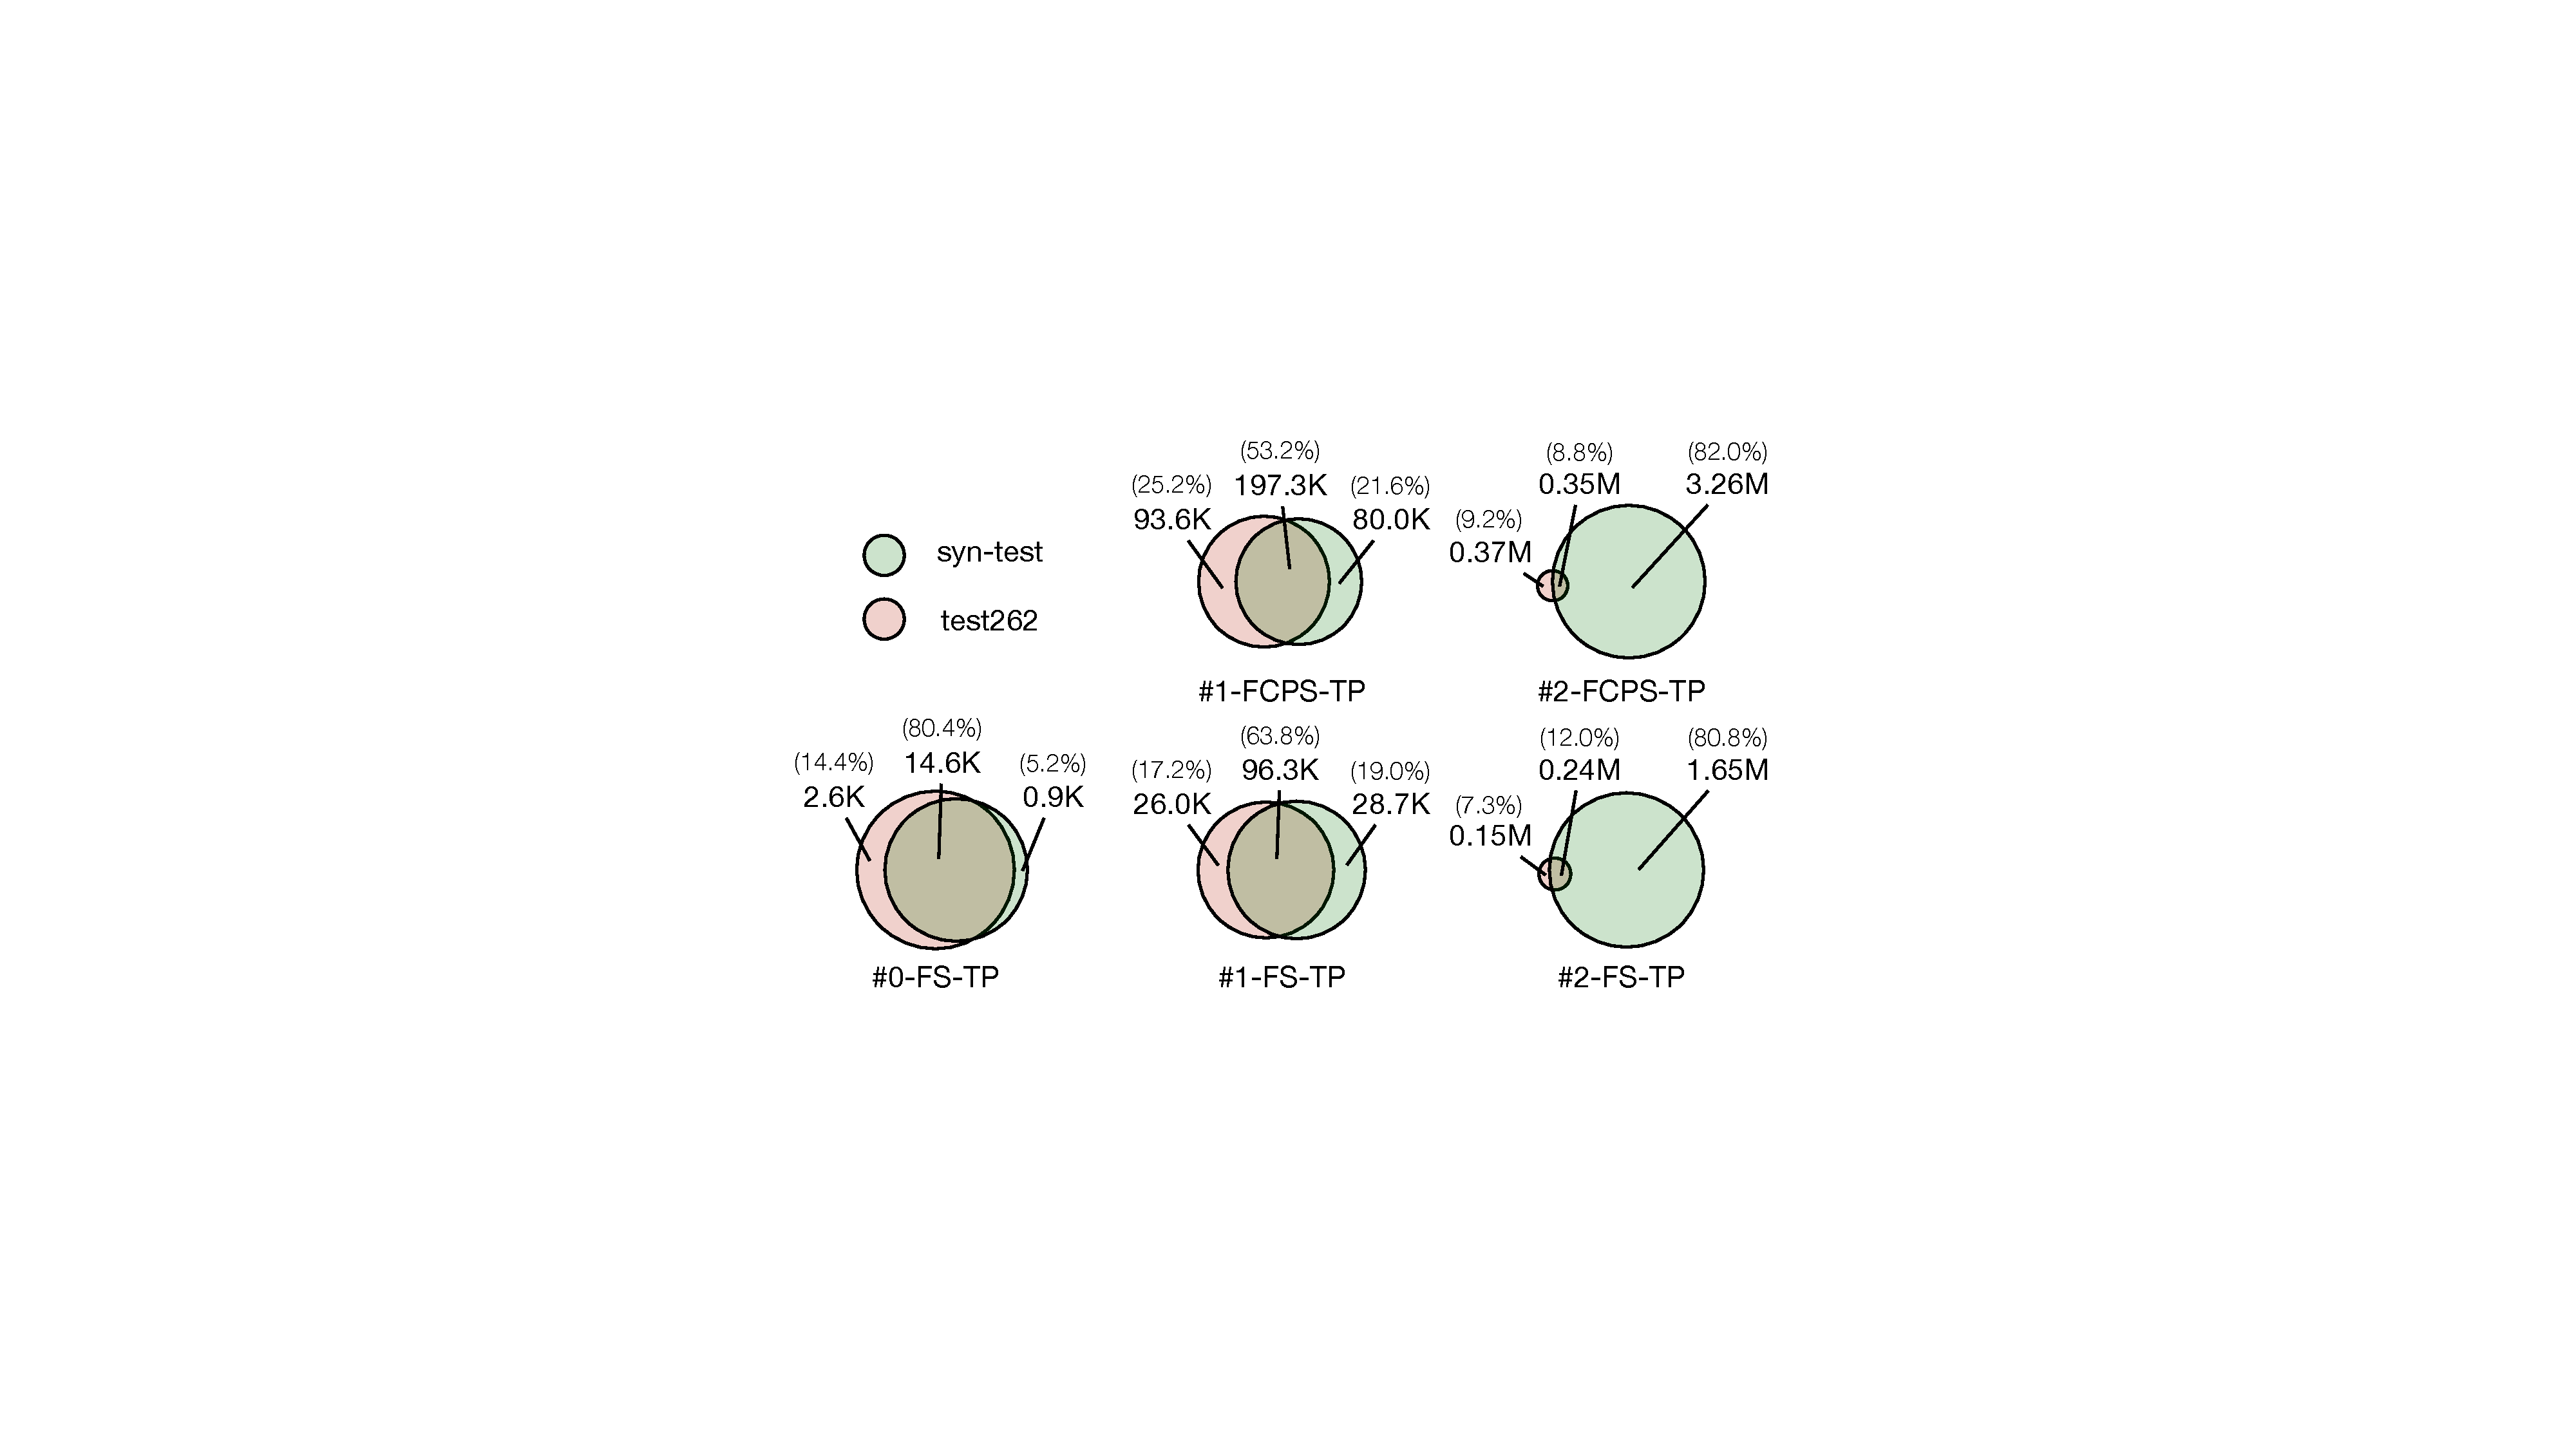
\includegraphics[width=\textwidth]{img/test262-venn}
    \caption{Covered TRs by synthesized tests and Test262}
  \end{subfigure}
%
  \begin{subfigure}{0.49\textwidth}
    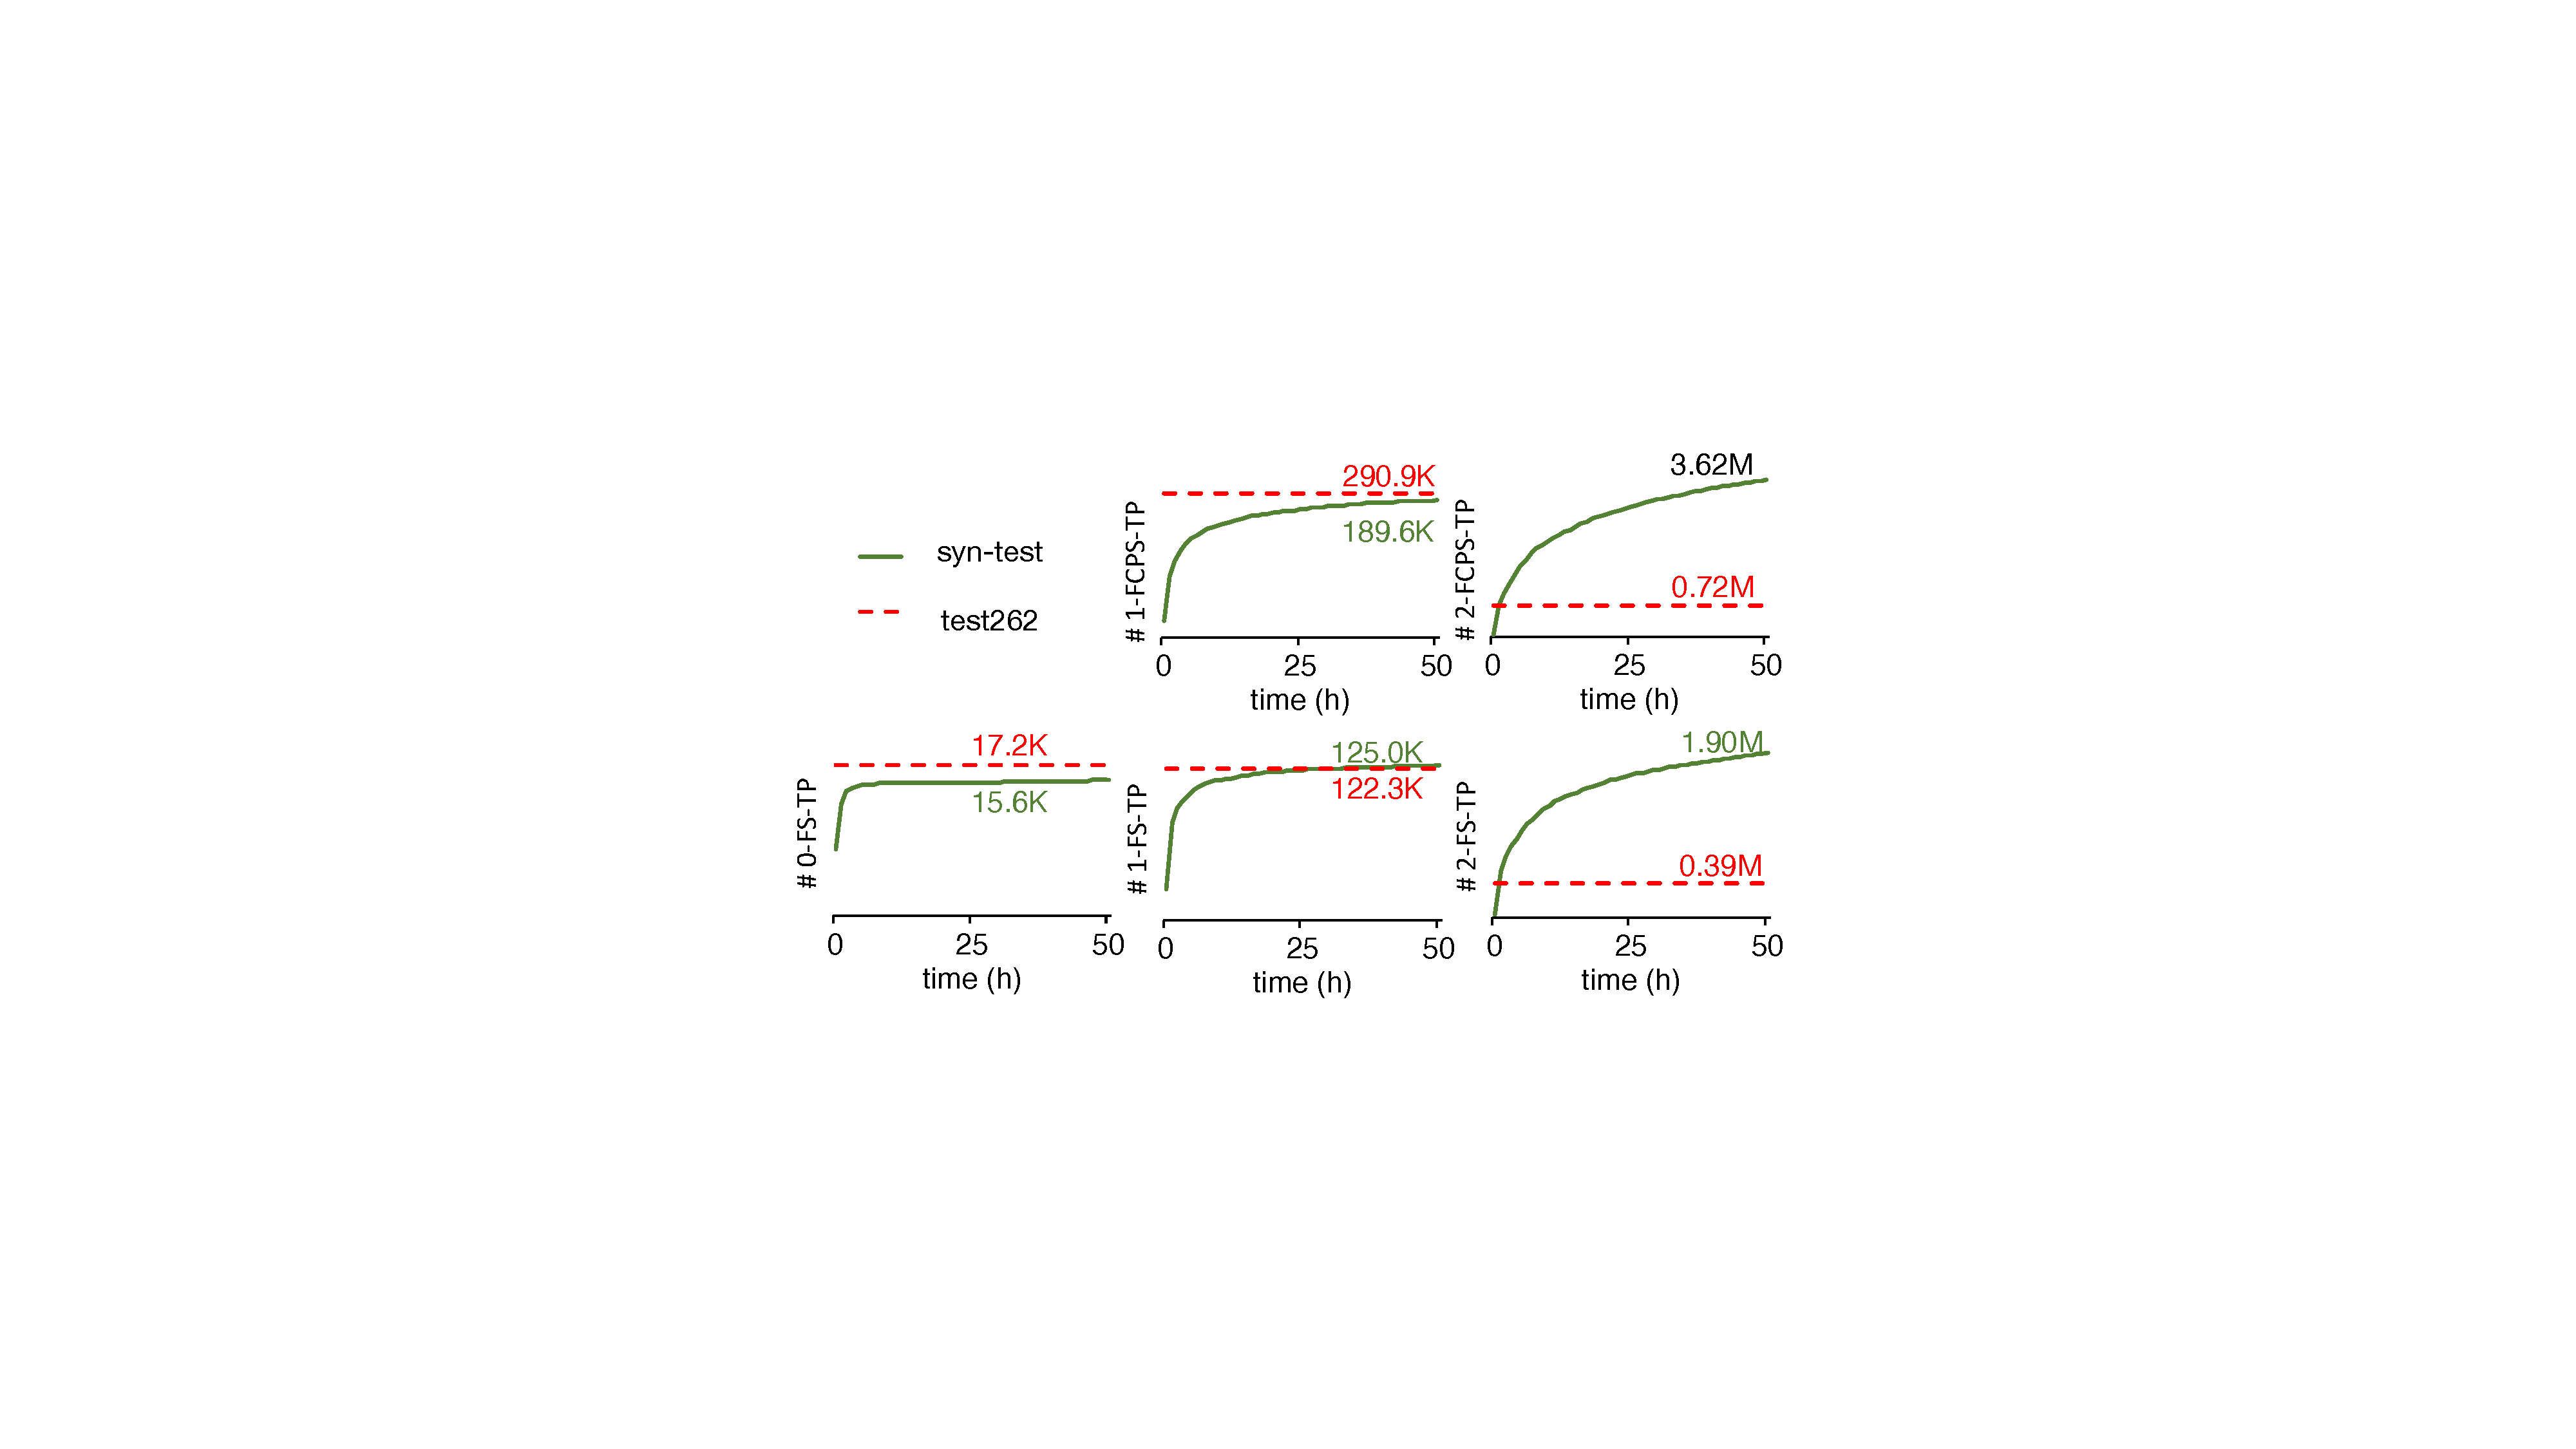
\includegraphics[width=\textwidth]{img/test262-time}
    \caption{Covered TRs over time}
  \end{subfigure}
%
  \caption{Covered $k$-FS-TRs and $k$-FCPS-TRs for synthesized tests via $\tool$ and Test262
  }
  \label{fig:test262}
\vspace*{-1em}
\end{figure}

%----------------------------------------%

We compare the coverage of automatically synthesized conformance tests with that
of Test262, the official JavaScript conformance test suite.
As described in Section~\ref{sec:impl}, the baseline tool $\jest$ relies on the
mechanized specification extracted by $\esmeta$.
Thus, we filter out conformance tests in Test262 that utilize language
features not supported in the extracted mechanized specification.
We use the conventional methodology in the literature~\cite{kjs, jiset, javert}
to remove inapplicable tests in Test262.
Then, we measured the coverage of 23,910 applicable Test262 conformance tests
with five $k$-FS and $k$-FCPS node-or-branch coverage criteria.


Figure~\ref{fig:test262} shows
(b) venn diagrams of
the numbers of covered $k$-FS-TRs and 
$k$-FCPS-TRs for the synthesized conformance tests (\sname{syn-test}) via
$\tool$ and applicable conformance tests in Test262 (\sname{test262}) and
(b) their changes over time.
Without any feature-sensitive coverages, the coverage of synthesized tests is
less than that of Test262, and only 5.2\% (0.9K) 0-FS-TRs are newly covered by
the synthesized tests.
%
On the other hand, the numbers of $k$-FS-TRs covered by only synthesized tests
increase when using higher $k$: 28.7K (19.0\%) for 1-FS-TRs and 1.65M (80.8\%)
for 2-FS-TRs.
%
In addition, the number of 1-FCPS-TRs (or 2-FCPS-TRs) covered by only
synthesized tests is higher than the number of 1-FS-TRs (or 2-FS-TRs)
covered by only synthesized tests:
80.0K (21.6\%) for 1-FCPS-TRs and 3.26M (82.0\%) for 2-FCPS-TRs.
Figure~\ref{fig:test262}(b) also shows that the coverage of Test262 is
better than that of synthesized tests without any feature-sensitive
coverages, but the coverage of synthesized tests outperforms that of
Test262 with $2$-FS-TRs and $2$-FCPS-TRs.
%
We believe that this is why $\tool$ successfully detected diverse new bugs in
existing JavaScript implementations, even though they have been heavily tested
using Test262 and various fuzzing techniques.

\section{Related Work}\label{sec:related}

\begin{itemize}
  \item JavaScript language specificaiton: ECMA-262 (ES13, 2022)~\cite{es13}
  \item JavaScript tests: Test262~\cite{test262}
  \item JavaScript tools: engines~\cite{v8, jscore, graaljs, chakra,
    spidermonkey, xs}, static analyzers~\cite{safe, safe2, tajs, wala, jsai},
    debugger~\cite{jsexplain}, verification tools~\cite{javert, javert2,
    ad-safety, javanni}, symbolic execution~\cite{symbolic-js, sym-js, expo-se},
    concolic testing~\cite{jalangi, type-conc-test}.
  \item Domain Specific Language (DSL)~\cite{dsl-survey, dsl-survey2}
  \item JISET family: $\jiset$~\cite{jiset}, $\jest$~\cite{jest},
    $\jstar$~\cite{jstar}, $\jsaver$~\cite{jsaver}.
  \item Partial Evaluation~\cite{peval, peval-survey}, Program
    Transformation~\cite{trans-ai}.
  \item JavaScript Engine Fuzzer~\cite{montage, langfuzz, die, favocado,
    codealchemist, sofi, comfort, superion, fuzzilli, jsfunfuzz,
  ifuzzer}.
\end{itemize}

\todo

\section{Conclusion}\label{sec:conclusion}
To support correct and consistent implementations of programming language semantics,
conformance testing using graph coverage has been one of the most
promising approaches. However, because language implementations often utilize 
different execution paths even for the same functionalities,
traditional graph coverage does not produce high-quality conformance tests.
In this paper, we present novel coverage criteria especially designed
for language implementations: \textit{feature-sensitive (FS) coverage} and
\textit{feature-call-path-sensitive (FCPS) coverage}
by refining conventional test requirements using
enclosing language features and call paths.
We also extend both coverage criteria using the $k$-limiting approach as
$k$-FS coverage and $k$-FCPS coverage.
Our experiments show that the new coverage criteria outperform the
traditional coverage criteria in the context of conformance bug detection in
real-world JavaScript implementations.
We detected \inred{115} distinct conformance bugs (\inred{40} in engines
and \inred{75} in transpilers), \inred{80} of which were confirmed by the
developers and \inred{40} of which were newly discovered bugs.


%% TODO acknowledgements
% \begin{acks}
% This work was supported by National Research Foundation of
% Korea (NRF) (Grants NRF-2017R1A2B3012020 and 2017M3C4A7068177).

%% bibliography style
\bibliographystyle{ACM-Reference-Format}

%% the bibliography file.
\balance
\bibliography{ref}

\end{document}
\endinput
